% Options for packages loaded elsewhere
\PassOptionsToPackage{unicode}{hyperref}
\PassOptionsToPackage{hyphens}{url}
\PassOptionsToPackage{dvipsnames,svgnames*,x11names*}{xcolor}
%
\documentclass[
  11pt,
]{article}
\usepackage{lmodern}
\usepackage{amssymb,amsmath}
\usepackage{ifxetex,ifluatex}
\ifnum 0\ifxetex 1\fi\ifluatex 1\fi=0 % if pdftex
  \usepackage[T1]{fontenc}
  \usepackage[utf8]{inputenc}
  \usepackage{textcomp} % provide euro and other symbols
\else % if luatex or xetex
  \usepackage{unicode-math}
  \defaultfontfeatures{Scale=MatchLowercase}
  \defaultfontfeatures[\rmfamily]{Ligatures=TeX,Scale=1}
\fi
% Use upquote if available, for straight quotes in verbatim environments
\IfFileExists{upquote.sty}{\usepackage{upquote}}{}
\IfFileExists{microtype.sty}{% use microtype if available
  \usepackage[]{microtype}
  \UseMicrotypeSet[protrusion]{basicmath} % disable protrusion for tt fonts
}{}
\makeatletter
\@ifundefined{KOMAClassName}{% if non-KOMA class
  \IfFileExists{parskip.sty}{%
    \usepackage{parskip}
  }{% else
    \setlength{\parindent}{0pt}
    \setlength{\parskip}{6pt plus 2pt minus 1pt}}
}{% if KOMA class
  \KOMAoptions{parskip=half}}
\makeatother
\usepackage{xcolor}
\IfFileExists{xurl.sty}{\usepackage{xurl}}{} % add URL line breaks if available
\IfFileExists{bookmark.sty}{\usepackage{bookmark}}{\usepackage{hyperref}}
\hypersetup{
  pdftitle={Supplemental Material: Declining Life Expectancy in the United States: Missing the Trees for the Forest},
  pdfauthor={Sam Harper1,2; Corinne A. Riddell3; Nicholas B. King1,2,4},
  colorlinks=true,
  linkcolor=Maroon,
  filecolor=Maroon,
  citecolor=Blue,
  urlcolor=blue,
  pdfcreator={LaTeX via pandoc}}
\urlstyle{same} % disable monospaced font for URLs
\usepackage[margin=1in]{geometry}
\usepackage{graphicx,grffile}
\makeatletter
\def\maxwidth{\ifdim\Gin@nat@width>\linewidth\linewidth\else\Gin@nat@width\fi}
\def\maxheight{\ifdim\Gin@nat@height>\textheight\textheight\else\Gin@nat@height\fi}
\makeatother
% Scale images if necessary, so that they will not overflow the page
% margins by default, and it is still possible to overwrite the defaults
% using explicit options in \includegraphics[width, height, ...]{}
\setkeys{Gin}{width=\maxwidth,height=\maxheight,keepaspectratio}
% Set default figure placement to htbp
\makeatletter
\def\fps@figure{htbp}
\makeatother
\setlength{\emergencystretch}{3em} % prevent overfull lines
\providecommand{\tightlist}{%
  \setlength{\itemsep}{0pt}\setlength{\parskip}{0pt}}
\setcounter{secnumdepth}{5}
\usepackage{booktabs}
\usepackage{sectsty}
\allsectionsfont{\bfseries\sffamily}
\renewcommand{\maketitlehooka}{\textsf}

\title{Supplemental Material: Declining Life Expectancy in the United States:
Missing the Trees for the Forest}
\author{Sam Harper\textsuperscript{1,2} \and Corinne A. Riddell\textsuperscript{3} \and Nicholas B. King\textsuperscript{1,2,4}}
\date{}

\begin{document}
\maketitle

\textsuperscript{1} Department of Epidemiology, Biostatistics \&
Occupational Health, McGill University, Montreal Canada\\
\textsuperscript{2} Institute for Health and Social Policy, McGill
University, Montreal, Canada\\
\textsuperscript{3} Division of Epidemiology \& Biostatistics, School of
Public Health, UC Berkeley, Berkeley, USA\\
\textsuperscript{4} Biomedical Ethics Unit, McGill University, Montreal,
Canada

\hypertarget{data-sources-and-methods}{%
\section{\textbar{} DATA SOURCES AND
METHODS}\label{data-sources-and-methods}}

\hypertarget{data}{%
\subsection{\textbar{} Data}\label{data}}

We used a number of data sources to construct plots and to analyze life
expectancy trends. Data on US life expectancy and life expectancy for
other Organization for Economic Cooperation and Development countries
were abstracted using the World Bank's World Development Indicators
online database (The World Bank Group 2020), specifically the series on
life expectancy at birth. For estimates within the US, the underlying
data source was the US National Vital Statistics System, maintained by
the \href{https://www.cdc.gov/nchs/index.htm}{National Center for Health
Statistics}, which collects information on all deaths occurring in the
United States each year.

Although NCHS collects data on race and gender, accurate mortality
statistics for the ``American Indian and Alaska Native'' group are
difficult to produce because of misclassification of Indigenous
individuals as white on death certificates. Thirty percent of deaths to
Indigenous individuals are estimated to be misclassified, hindering
abilities to calculate life expectancy or calculate accurate,
cause-specific mortality rates. In 2008, Arias and colleagues (Arias et
al. 2008) adjusted for misreporting of Indigenous ethnicity and
estimated life expectancy for this group to be 71.1, 2.8 years lower
than the next-lowest life expectancy estimate for Non-Hispanic Blacks.
The age-adjusted mortality rate from opioid overdoses (not adjusted for
ethnicity misreporting) was estimated to be between the mortality rates
for non-Hispanic whites and non-Hispanic blacks during 2017 (Woolf and
Schoomaker 2019). Even with under-reporting Indigenous Americans have
the highest reported rates of suicide, and the second-highest reported
rate of homicide (Kochanek et al. 2019). A more recent update by Arias
and colleagues (Arias et al. 2016) that the quality of reporting for the
American Indian and Alaska Native population remains poor. For these
reasons we were unable to estimate life expectancy and cause-specific
mortality for this population.

\hypertarget{cdc-wonder}{%
\subsubsection{\textbar{} CDC WONDER}\label{cdc-wonder}}

We extracted mortality data by age, gender, and cause of death for
various analyses using the CDC's Wide-ranging Online Data for
Epidemiologic Research, called \href{https://wonder.cdc.gov/}{WONDER}
(Centers for Disease Control and Prevention and National Center for
Health Statistics 2020). We used the ``Underlying Cause of Death
1999-2018''
\href{https://wonder.cdc.gov/wonder/help/ucd.html\#}{database} to
generate mortality trends by age, gender, race, ethnicity, and
cause-of-death, as well as geography for some figures.

\hypertarget{seer-stat}{%
\subsubsection{\textbar{} SEER Stat}\label{seer-stat}}

In addition to CDC WONDER we also used the SEER*Stat interface (National
Cancer Institute 2019) to produce some mortality rates that were more
difficult to do using CDC WONDER, such as age-adjusted rates within
broad age categories, as well as longer term trends for some causes of
death. However, the underlying data for SEER*Stat are also maintained
and produced by NCHS. See the mortality documentation at the SEER*Stat
\href{https://seer.cancer.gov/mortality/}{website}.

\hypertarget{estimation-of-life-expectancy-and-decomposition}{%
\subsection{\textbar{} Estimation of life expectancy and
decomposition}\label{estimation-of-life-expectancy-and-decomposition}}

We used standard methods for creating abridged life tables (Preston,
Heuveline, and Guillot 2001), with 11 10-year age groups (0-1, 1-4,
5-14, \ldots{} , 85+). We calculated the contribution of each age group
and cause-of-death to the difference in life expectancy between the
years 2014 and 2017 using the methods developed by Arriaga (Arriaga
1984). Briefly, the contribution of a particular age group is both a
direct function of the difference in age-specific mortality rates at
that age plus an additional contribution resulting from the fact that
mortality differences at a given age will produce additional survivors
at older ages (Arriaga 1984), given by the formula below:

\[ _{n}\Delta_{x}=\left[\underbrace{l_{x}^{2017}/l_{0}^{2017}}_{\textrm{fraction of survivors}}\times\overbrace{\left(\dfrac{_{n}L_{x}^{2014}}{l_{x}^{2014}}-\dfrac{_{n}L_{x}^{2017}}{l_{x}^{2017}}\right)}^{\textrm{direct effect}}\right]+\overbrace{\left[\dfrac{T_{x+n}^{2014}}{l_{x+n}^{2014}}\times\dfrac{\dfrac{l_{x}^{2017}l_{x+n}^{2014}}{l_{x}^{2014}}-l_{x+n}^{2017}}{l_{0}^{2017}}\right]}^{\textrm{indirect effect + interaction}} \]
where \(_{n}\Delta_{x}\) is the total contribution for a given age
interval between \(x\) and \(x+n\), \(l_{x}\) is number alive at age
\(x\), \(L_{x}\) is the person-years lived in the interval, and
\(T_{x}\) is the person-time lived beyond age \(x\).

The contribution \(_{n}\Delta_{x}^{i}\) of each cause of death \(i\)
within a given age group is a function of the difference between the two
time periods in the proportion of deaths due to a given cause (Arriaga
1989):

\[
_{n}\Delta_{x}^{i}={}_{n}\Delta_{x}\times\dfrac{\overbrace{\left(_{n}p_{x}^{i,2014}\times{}_{n}r_{x}^{2014}\right)-\left(_{n}p_{x}^{i,2017}\times{}_{n}r_{x}^{2017}\right)}^{\textrm{difference in share of deaths for cause}\,i}}{\underbrace{_{n}r_{x}^{2014}-_{n}r_{x}^{2017}}_{\textrm{overall mortality rate difference}}}
\]

where \(_{n}\Delta_{x}\) is the total contribution for an age group,
\(_{n}p_{x}^{i}\) is the proportion of deaths within age group \(x\) due
to cause \(i\), and \(_{n}r_{x}\) is the overall age-specific death
rate. The total difference in life expectancy is the net sum of the
age-cause components:

\[
\sum_{i}{}_{n}\Delta_{x}^{i}={}_{n}\Delta_{x},\:\textrm{and}\:e_{0}^{2014}-e_{0}^{2017}=\sum_{x}{}_{n}\Delta_{x}=\sum_{x}\sum_{i}{}_{n}\Delta_{x}^{i}
\]

The total difference in life expectancy at birth between 2017 and 2014
is the sum of the age-cause specific components. The total contribution
of a given age group to the difference in life expectancy is equal to
the sum of its contributions across all causes of death. Likewise, the
contribution of a particular cause of death is the sum of its
contributions across age groups.

\hypertarget{joinpoint-analysis-of-life-expectancy-trends}{%
\subsection{\textbar{} Joinpoint analysis of life expectancy
trends}\label{joinpoint-analysis-of-life-expectancy-trends}}

We also used joinpoint regression software (National Cancer Institute
2020) to examine when trends in life expectancy and mortality may have
changed in recent years. This was used to produce the estiamtes of
changes in US life expectancy relative to OECD countries, as well as for
the estimates of US life expectancy trends by gender and race-ethnicity.
This program uses segmented weighted least squares regression and
iteratively adds up to 5 segments and uses a permutation test (Kim et
al. 2000) to select the model that best fits the observed data.

\hypertarget{supplemental-tables-and-figures}{%
\section{\textbar{} SUPPLEMENTAL TABLES AND
FIGURES}\label{supplemental-tables-and-figures}}

The data and code to reproduce these tables and figures are provided via
the links in each caption, as well as in a public repository at the Open
Science Foundation: \url{https://osf.io/ypwfh/}.

\newpage

\textbf{Supplemental Table 1.} Life expectancy by gender and
race-ethnicity, 1999-2018. Source: Authors' calculations of data from
CDC WONDER (Centers for Disease Control and Prevention and National
Center for Health Statistics 2020). Data: \url{https://osf.io/y4fzx/},
\url{https://osf.io/wsdvb/} Code: \url{https://osf.io/ewxm7/}

\begin{table}[h]
\begin{tabular}{@{}llllllllllll@{}}
\toprule
          & \multicolumn{2}{l}{Non-Hispanic API} &  & \multicolumn{2}{l}{Non-Hispanic Black} &  & \multicolumn{2}{l}{Non-Hispanic White} &  & \multicolumn{2}{l}{Hispanic} \\ \cmidrule(lr){2-3} \cmidrule(lr){5-6} \cmidrule(lr){8-9} \cmidrule(l){11-12} 
Year      & Women             & Men              &  & Women              & Men               &  & Women              & Men               &  & Women         & Men          \\ \midrule
1999      & 86.6              & 81.3             &  & 74.9               & 67.8              &  & 79.8               & 74.7              &  & 83.0          & 77.2         \\
2000      & 87.0              & 81.6             &  & 75.0               & 68.1              &  & 79.9               & 74.8              &  & 83.3          & 77.4         \\
2001      & 87.1              & 82.0             &  & 75.3               & 68.4              &  & 79.9               & 74.9              &  & 83.3          & 77.6         \\
2002      & 87.3              & 82.2             &  & 75.3               & 68.6              &  & 79.9               & 74.9              &  & 83.5          & 77.7         \\
2003      & 87.4              & 82.5             &  & 75.5               & 68.8              &  & 80.0               & 75.1              &  & 83.6          & 77.9         \\
2004      & 87.8              & 83.1             &  & 76.0               & 69.3              &  & 80.4               & 75.5              &  & 84.2          & 78.6         \\
2005      & 87.9              & 82.9             &  & 76.1               & 69.4              &  & 80.4               & 75.5              &  & 84.1          & 78.2         \\
2006      & 88.1              & 83.3             &  & 76.6               & 69.8              &  & 80.6               & 75.8              &  & 84.4          & 78.9         \\
2007      & 88.5              & 83.8             &  & 77.0               & 70.2              &  & 80.9               & 76.0              &  & 84.9          & 79.3         \\
2008      & 88.3              & 84.0             &  & 77.3               & 70.9              &  & 80.8               & 76.0              &  & 84.8          & 79.7         \\
2009      & 88.7              & 84.2             &  & 77.8               & 71.4              &  & 81.2               & 76.4              &  & 85.4          & 80.1         \\
2010      & 88.8              & 84.1             &  & 78.1               & 71.8              &  & 81.2               & 76.5              &  & 85.4          & 80.2         \\
2011      & 89.2              & 84.7             &  & 78.3               & 72.2              &  & 81.2               & 76.5              &  & 85.8          & 80.8         \\
2012      & 89.1              & 84.8             &  & 78.6               & 72.3              &  & 81.3               & 76.6              &  & 85.8          & 80.9         \\
2013      & 89.5              & 84.7             &  & 78.6               & 72.4              &  & 81.3               & 76.6              &  & 86.0          & 81.0         \\
2014      & 90.0              & 85.5             &  & 78.8               & 72.7              &  & 81.3               & 76.6              &  & 86.3          & 81.3         \\
2015      & 89.7              & 85.4             &  & 78.8               & 72.4              &  & 81.1               & 76.5              &  & 86.3          & 81.2         \\
2016      & 89.7              & 85.5             &  & 78.6               & 72.1              &  & 81.2               & 76.3              &  & 86.4          & 81.1         \\
2017      & 89.7              & 85.3             &  & 78.8               & 72.0              &  & 81.1               & 76.3              &  & 86.4          & 81.1         \\
2018      & 90.0              & 85.5             &  & 78.8               & 72.0              &  & 81.3               & 76.4              &  & 86.5          & 81.0         \\
Changes   &                   &                  &  &                    &                   &  &                    &                   &  &               &              \\
2014-2017 & -0.3              & -0.2             &  & 0.0                & -0.7              &  & -0.2               & -0.3              &  & 0.1           & -0.2         \\
2010-2018 & 1.2               & 1.4              &  & 0.7                & 0.2               &  & 0.1                & -0.1              &  & 1.1           & 0.8          \\ \bottomrule
\end{tabular}
\end{table}

\newpage

\textbf{Supplemental Figure 1.} Life expectancy at birth in the United
States and 29 other high-income countries, 1969-2017. Source: World
Development Indicators (The World Bank Group 2020). Data:
\url{https://osf.io/d2b7c/}, \url{https://osf.io/n4mj6/} Code:
\url{https://osf.io/muyrk/}

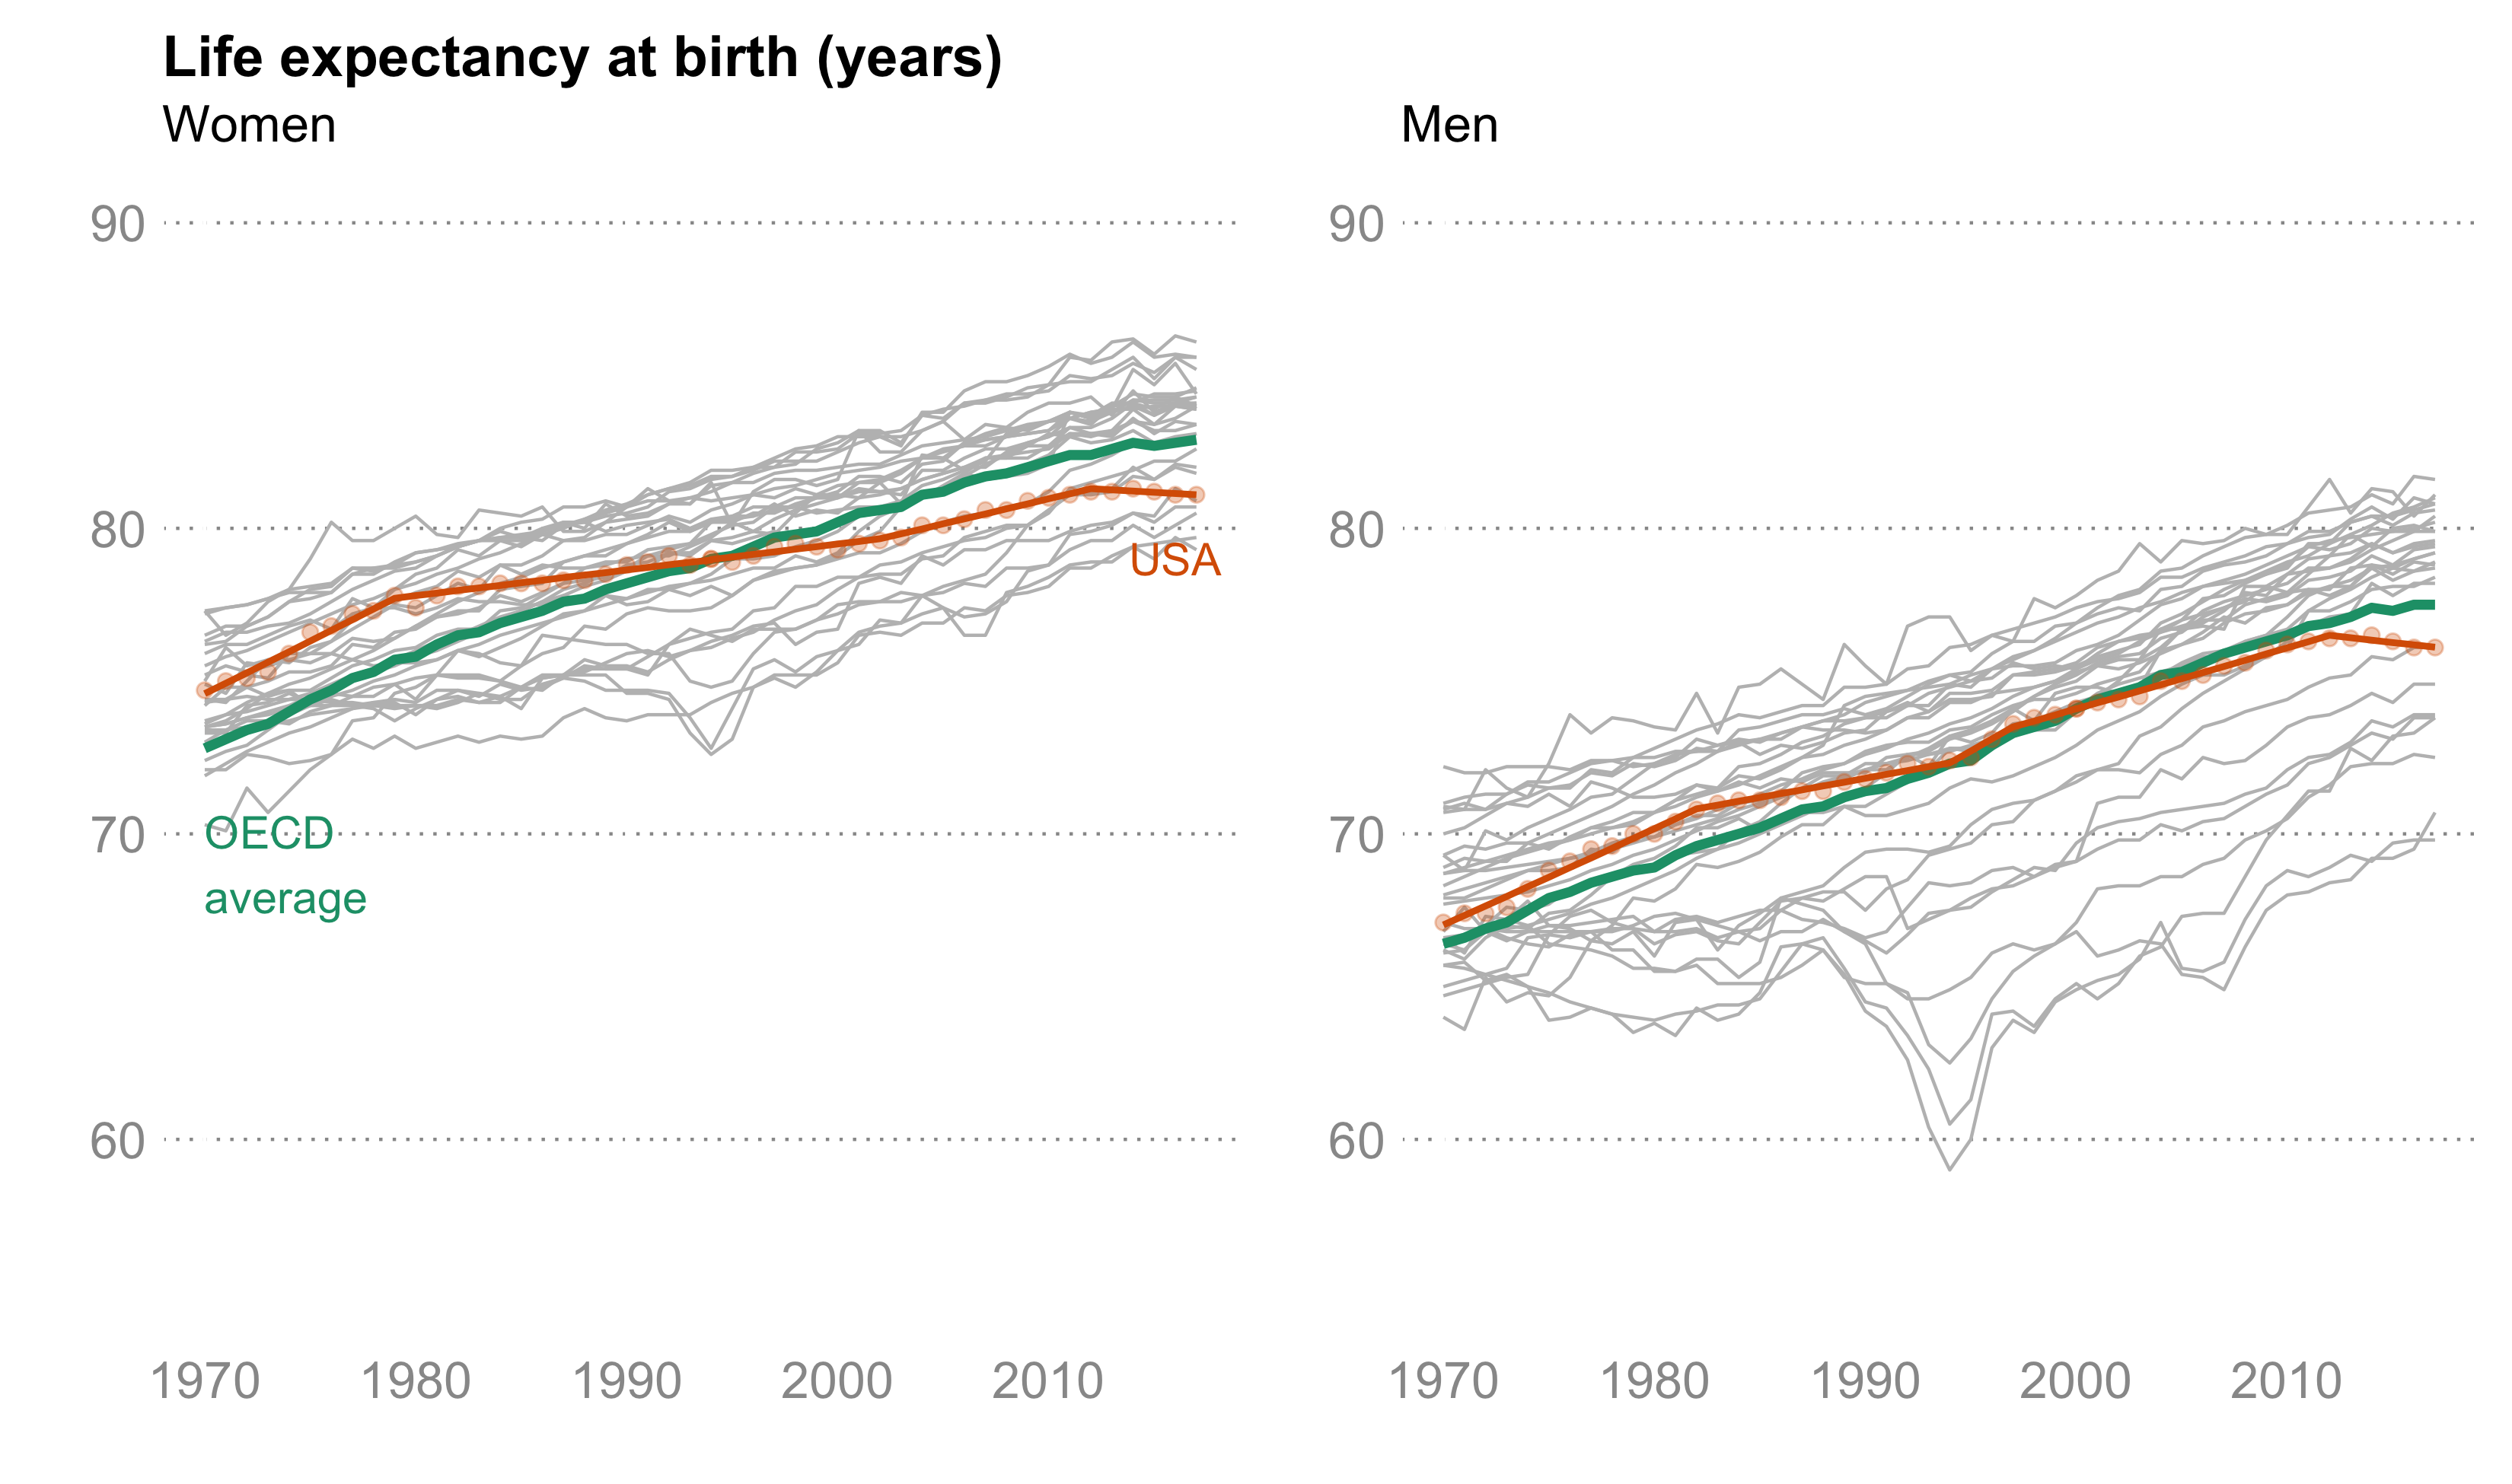
\includegraphics[width=1\linewidth]{../figures/us-le-trends-gender}

\newpage

\textbf{Supplemental Figure 2.} Annual year-on-year change in life
expectancy, USA and average of 29 other OECD countries. Source: World
Development Indicators (The World Bank Group 2020). Data:
\url{https://osf.io/d2b7c/}, \url{https://osf.io/n4mj6/} Code:
\url{https://osf.io/muyrk/}

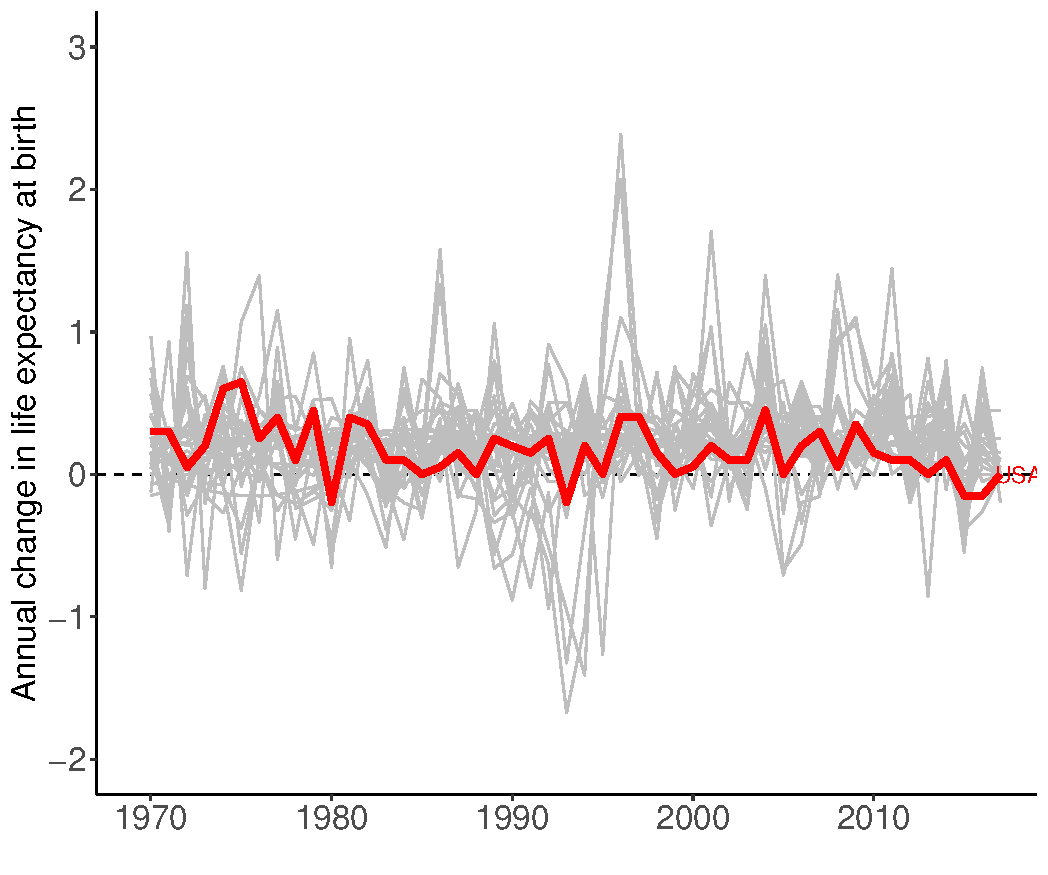
\includegraphics[width=1\linewidth]{../figures/us-le-change}

\newpage

\textbf{Supplemental Figure 3.} Trends the gender gap in life expectancy
by age and race-ethnicity, 1999-2018. Source: Authors' calculations of
data from CDC WONDER (Centers for Disease Control and Prevention and
National Center for Health Statistics 2020). Data:
\url{https://osf.io/4s2rz/} Code: \url{https://osf.io/5xywp/}

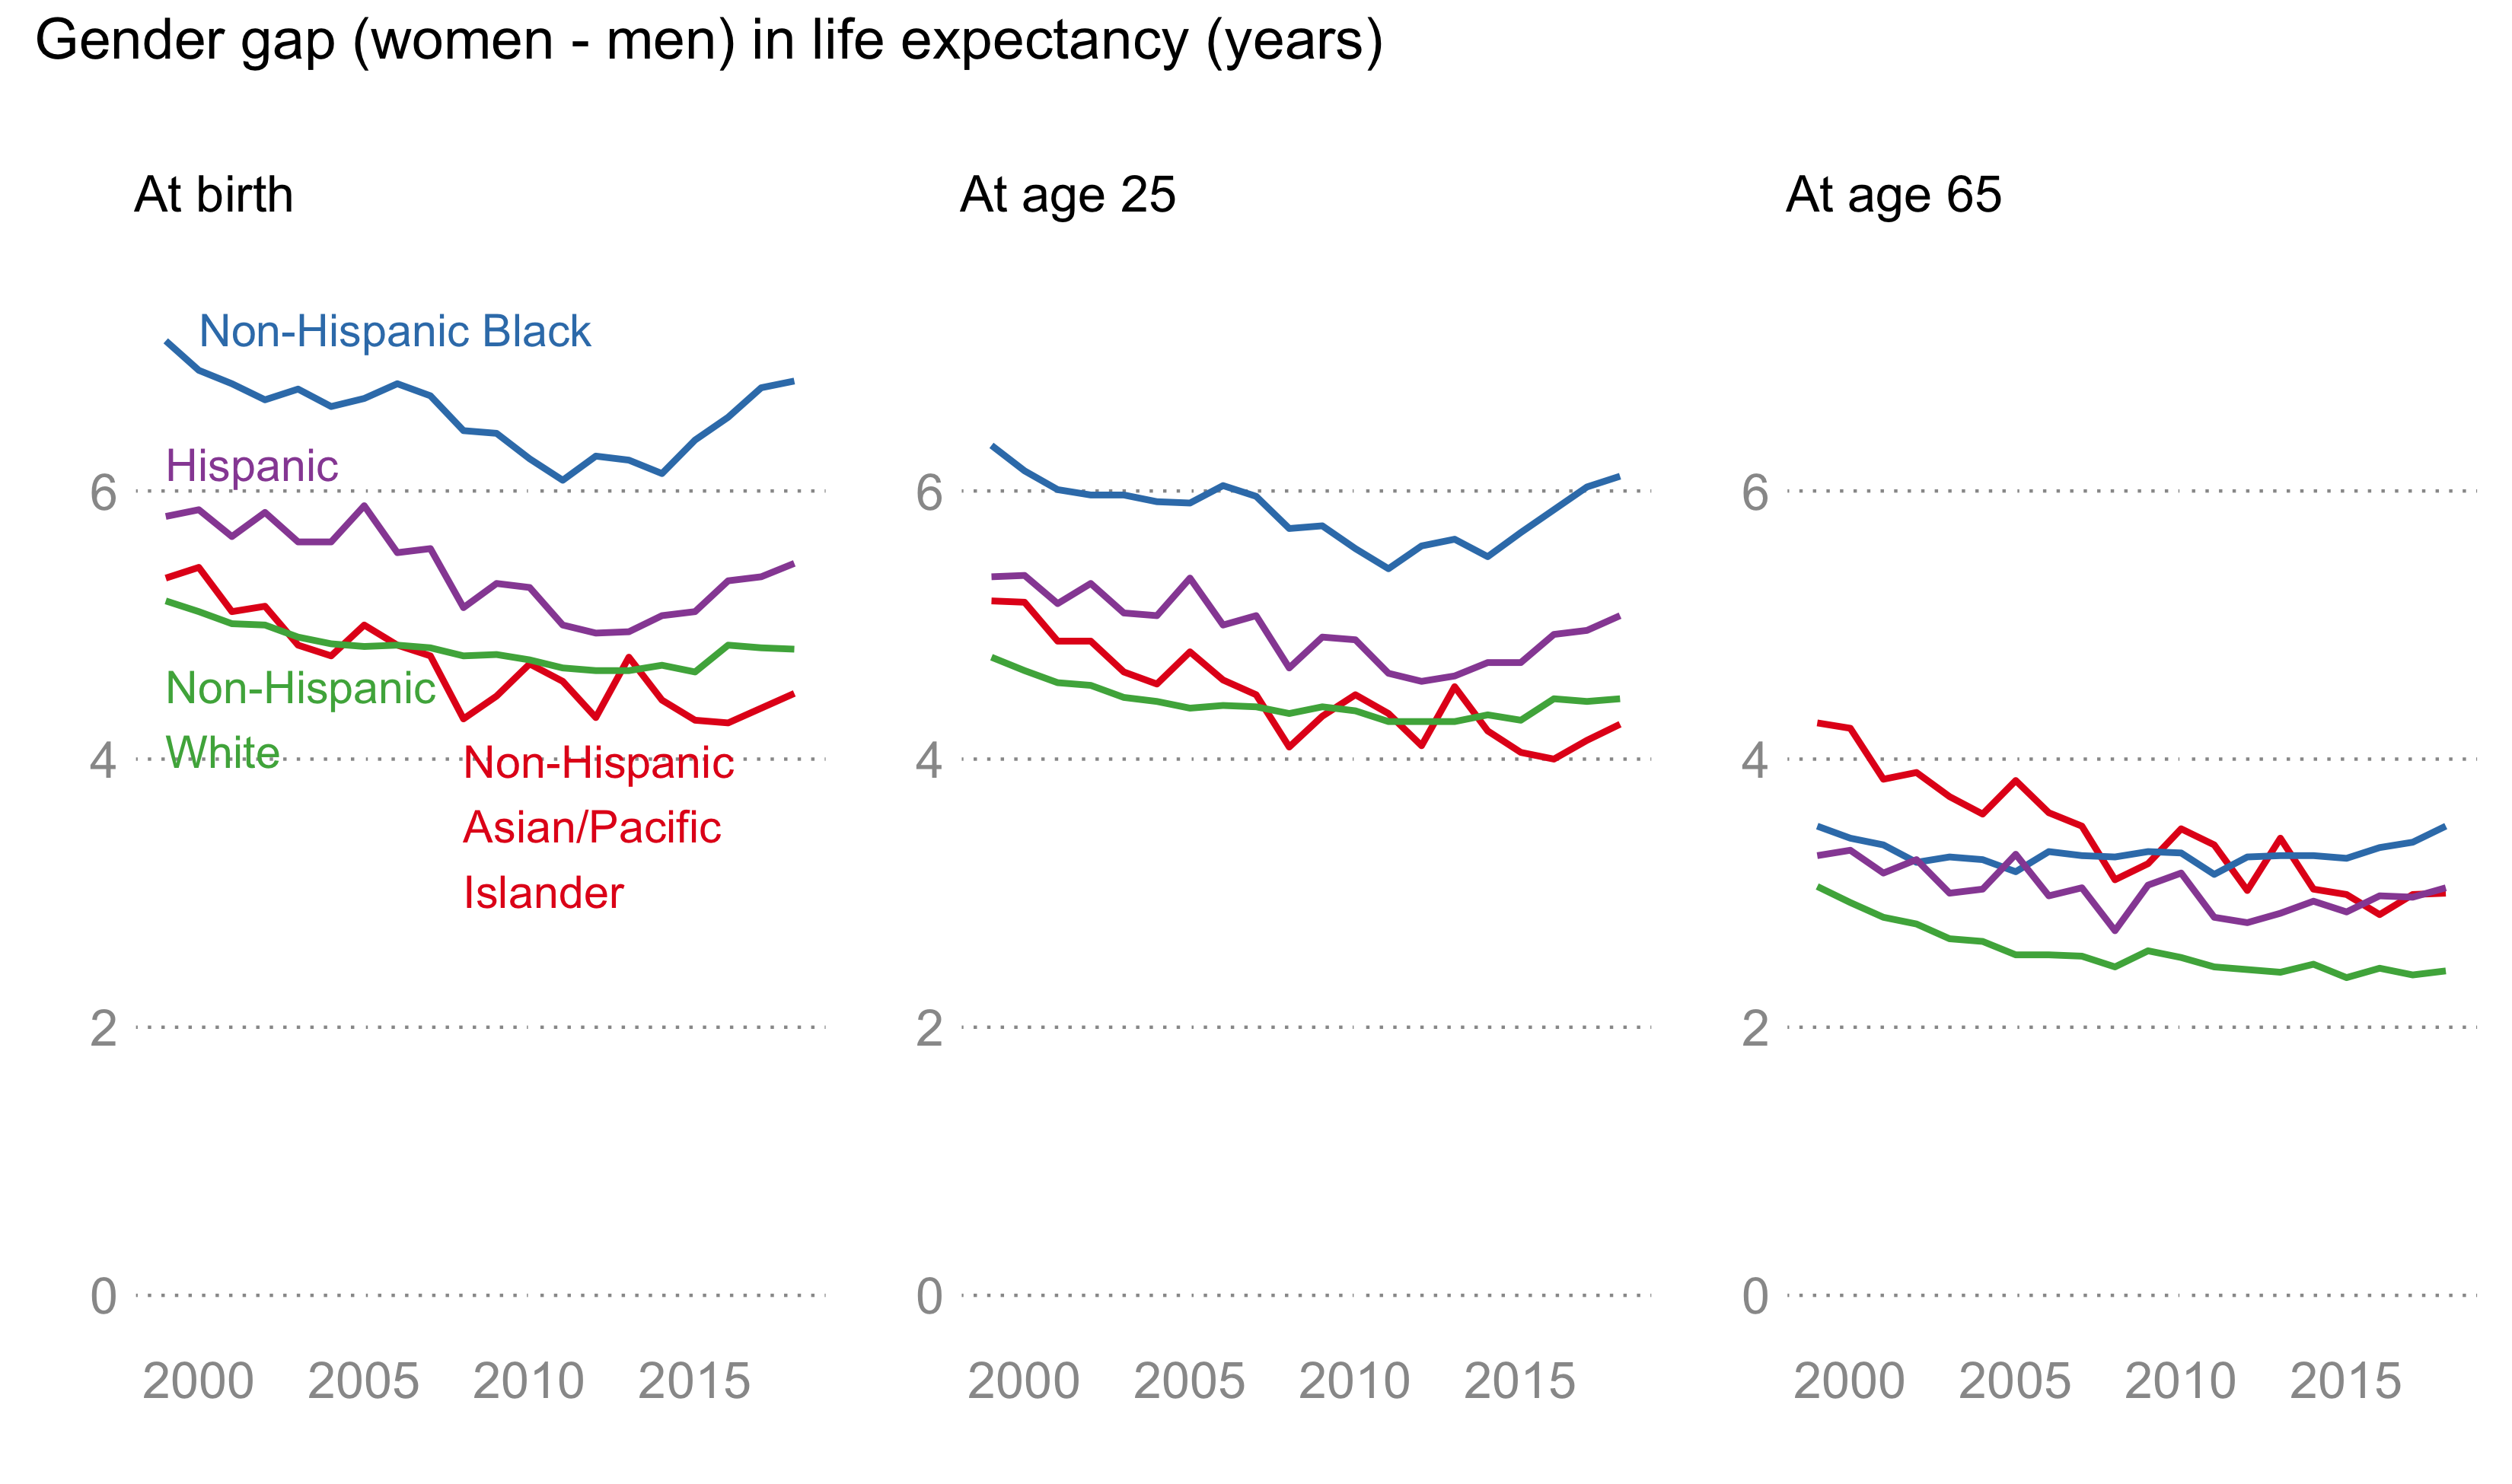
\includegraphics[width=1\linewidth]{../figures/le-gender-gap}

\newpage

\textbf{Supplemental Figure 4.} Life expectancy at age 25 and age 65 in
the United States, by gender and race-ethnicity, 1999-2018. Source:
Authors' calculations of data from CDC WONDER (Centers for Disease
Control and Prevention and National Center for Health Statistics 2020).
Data: \url{https://osf.io/hz864/} \url{https://osf.io/4s2rz/} Code:

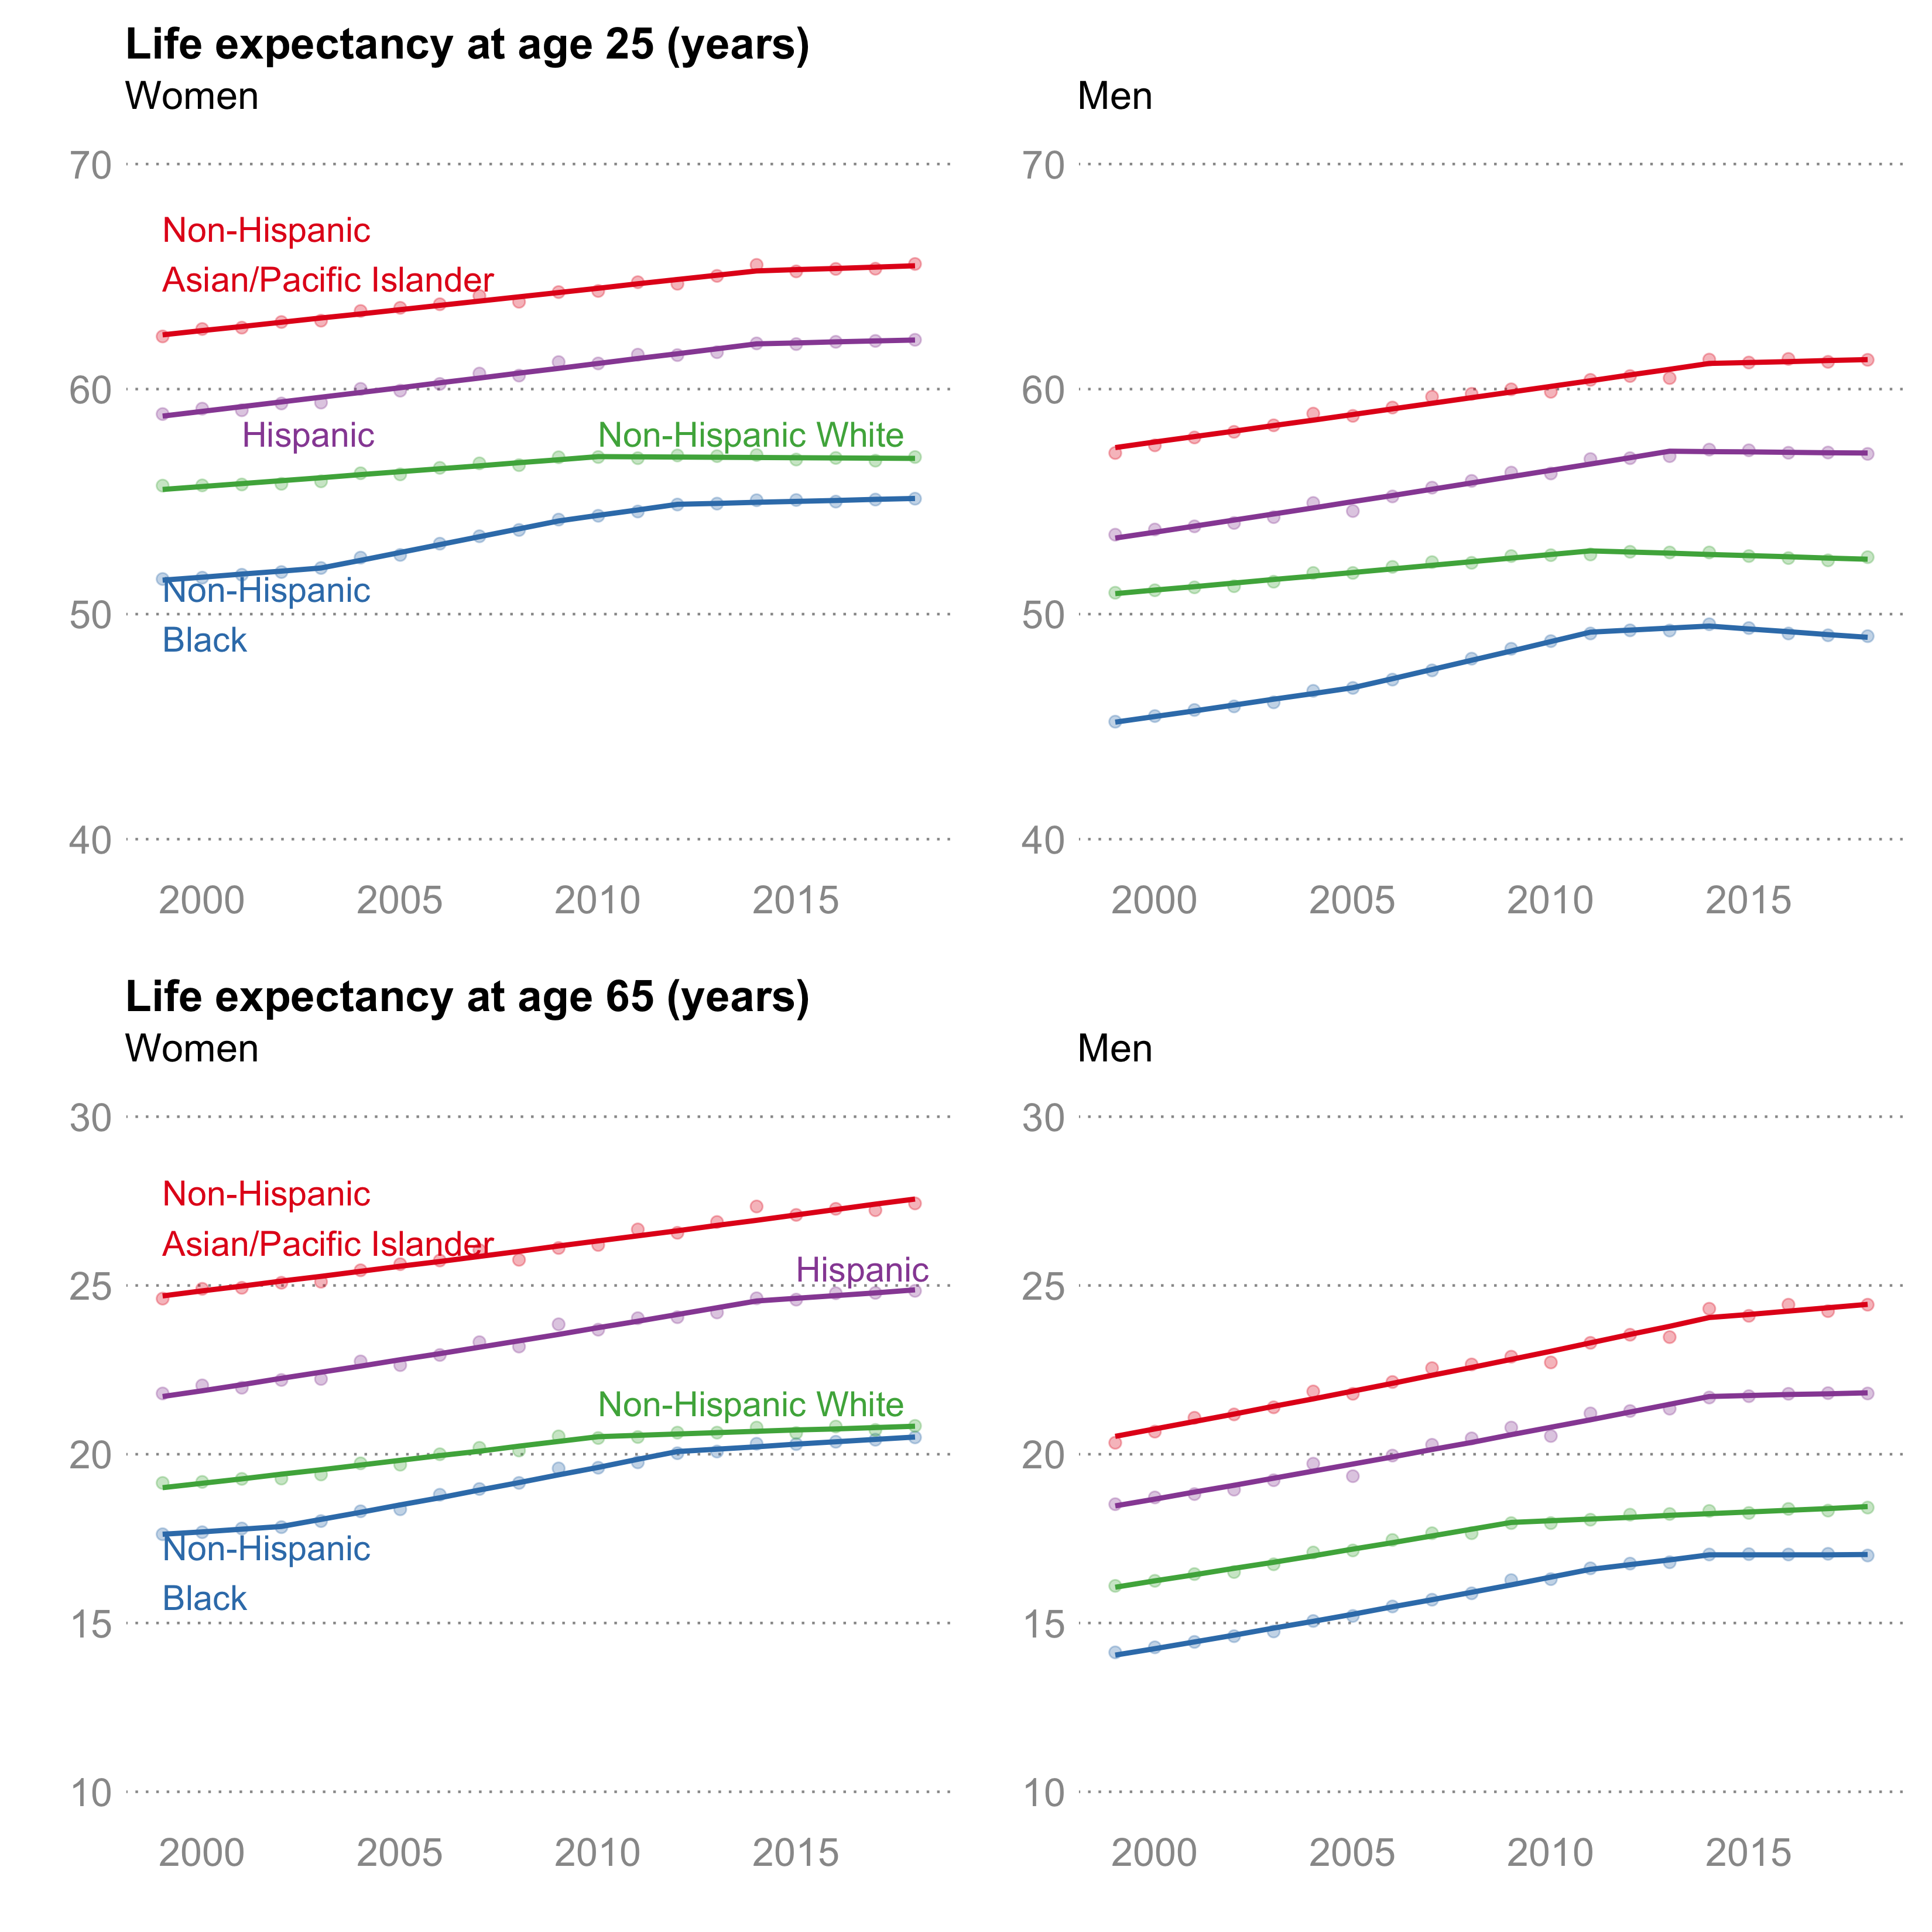
\includegraphics[width=1\linewidth]{../figures/le-jp2565}

\newpage

\textbf{Supplemental Figure 5.} Mortality rates by single years of age
by race-ethnicity for women, ages 25-64. Source: Authors' calculations
of data from CDC WONDER (Centers for Disease Control and Prevention and
National Center for Health Statistics 2020). Data:
\url{https://osf.io/uvyx4/}, \url{https://osf.io/pytev/} Code:
\url{https://osf.io/vb28p/}

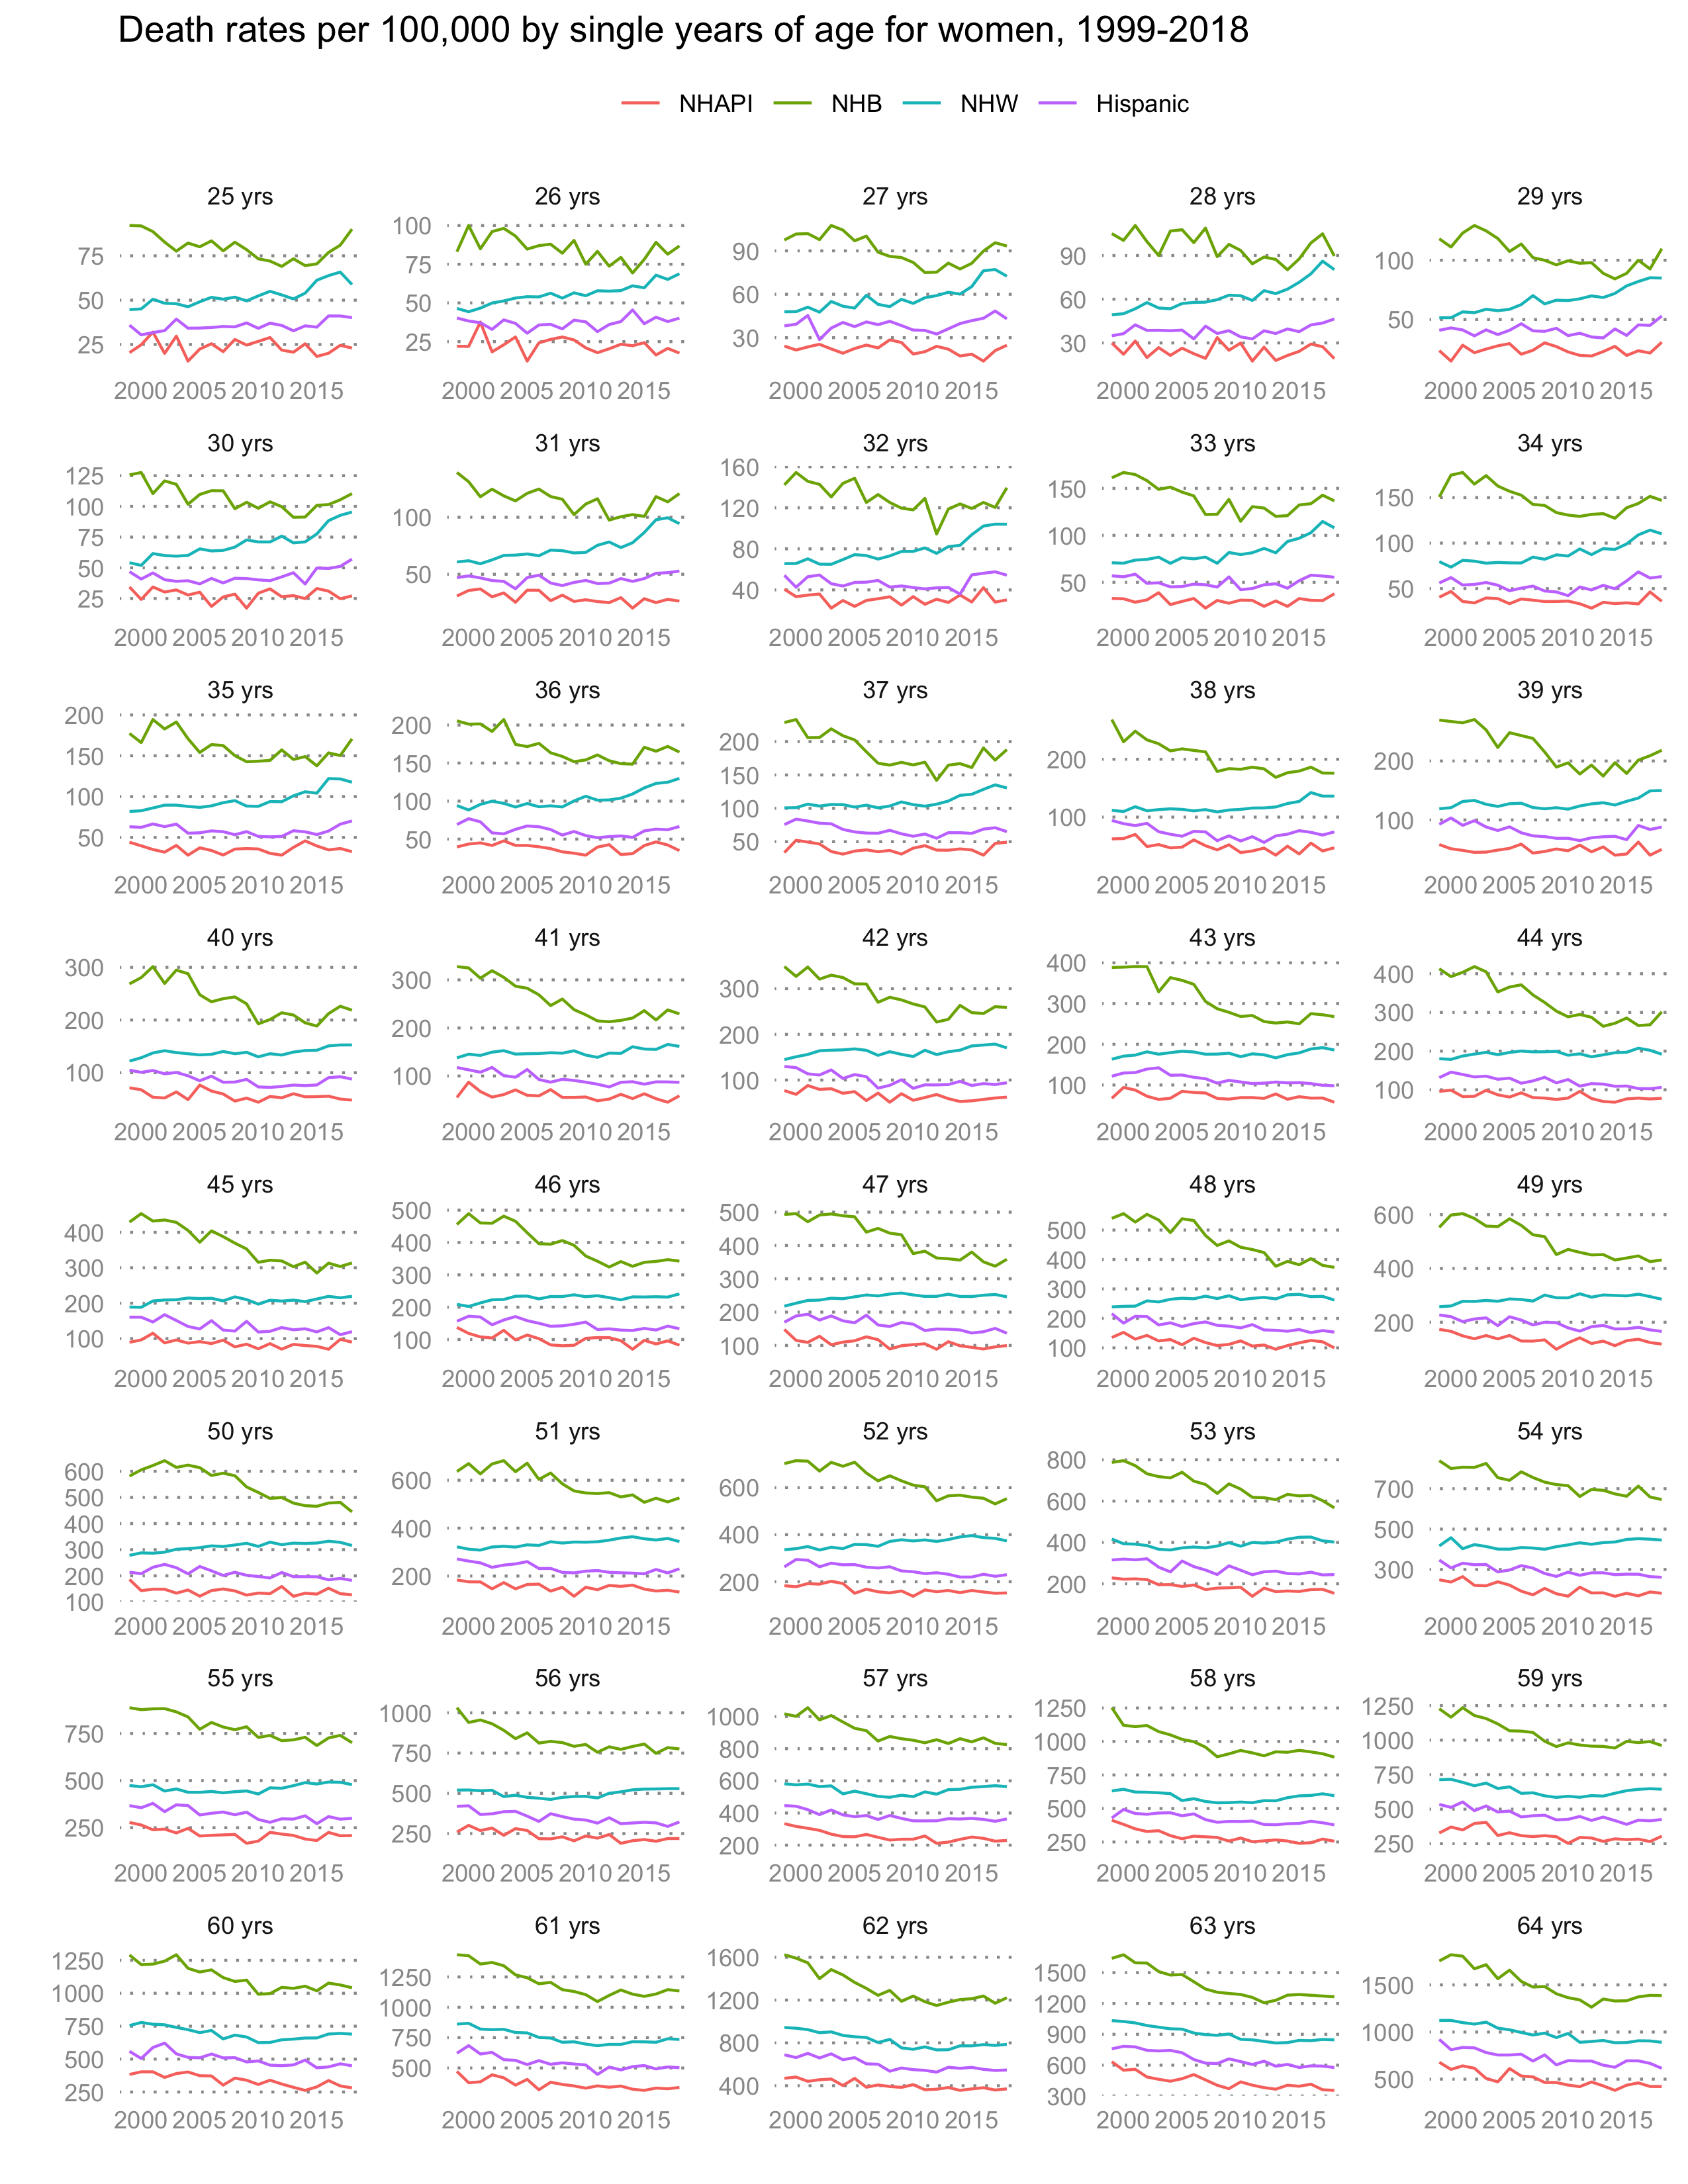
\includegraphics[width=0.9\linewidth]{../figures/single-ages-women}

\newpage

\textbf{Supplemental Figure 6.} Mortality rates by single years of age
by race-ethnicity for men, ages 25-64. Source: Authors' calculations of
data from CDC WONDER (Centers for Disease Control and Prevention and
National Center for Health Statistics 2020). Data:
\url{https://osf.io/uvyx4/}, \url{https://osf.io/pytev/} Code:
\url{https://osf.io/vb28p/}

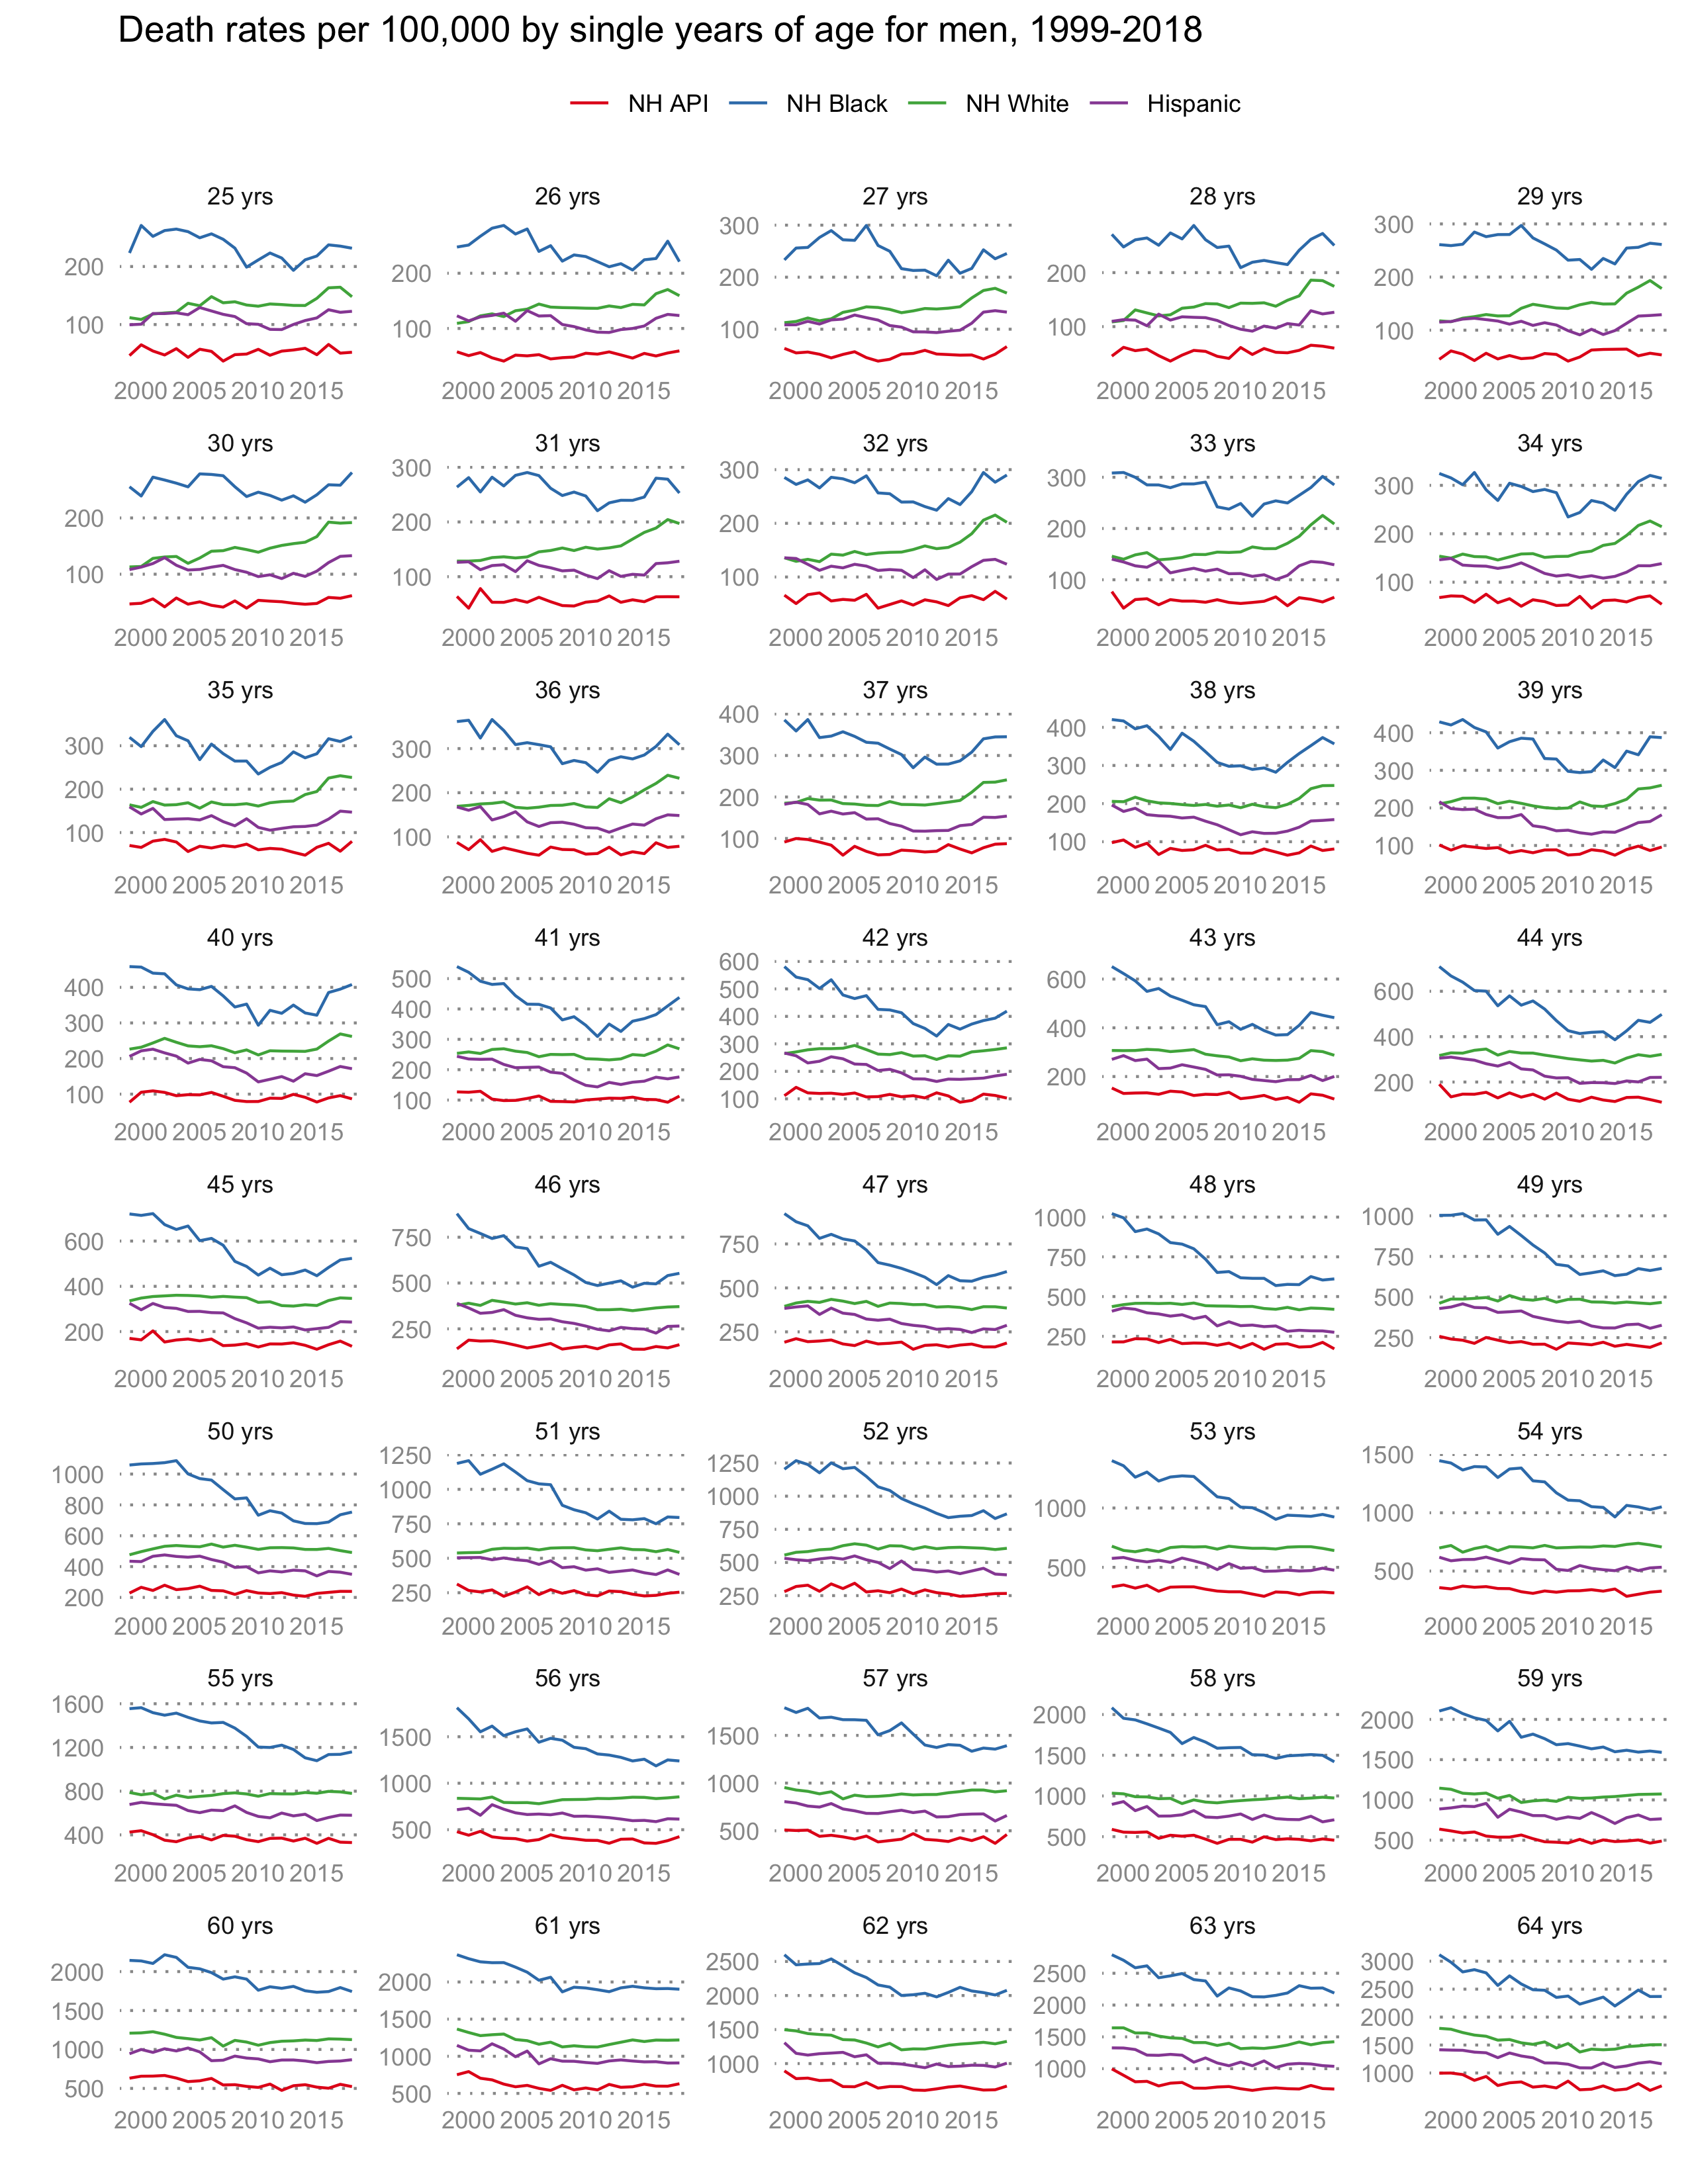
\includegraphics[width=0.9\linewidth]{../figures/single-ages-men}

\newpage

\textbf{Supplemental Figure 7.} Age groups contributing to the change in
life expectancy at birth in the United States between 2010 and 2018, by
gender and race-ethnicity. Red color indicates age groups contributing a
decline, blue color indicates age groups contributing an increase.
Source: Authors' calculations of data from CDC WONDER (Centers for
Disease Control and Prevention and National Center for Health Statistics
2020). Data: \url{https://osf.io/tk8q3/}, \url{https://osf.io/mctx3/}
\url{https://osf.io/utdnv/} Code: \url{https://osf.io/g9mp2/},
\url{https://osf.io/qd5w4/}

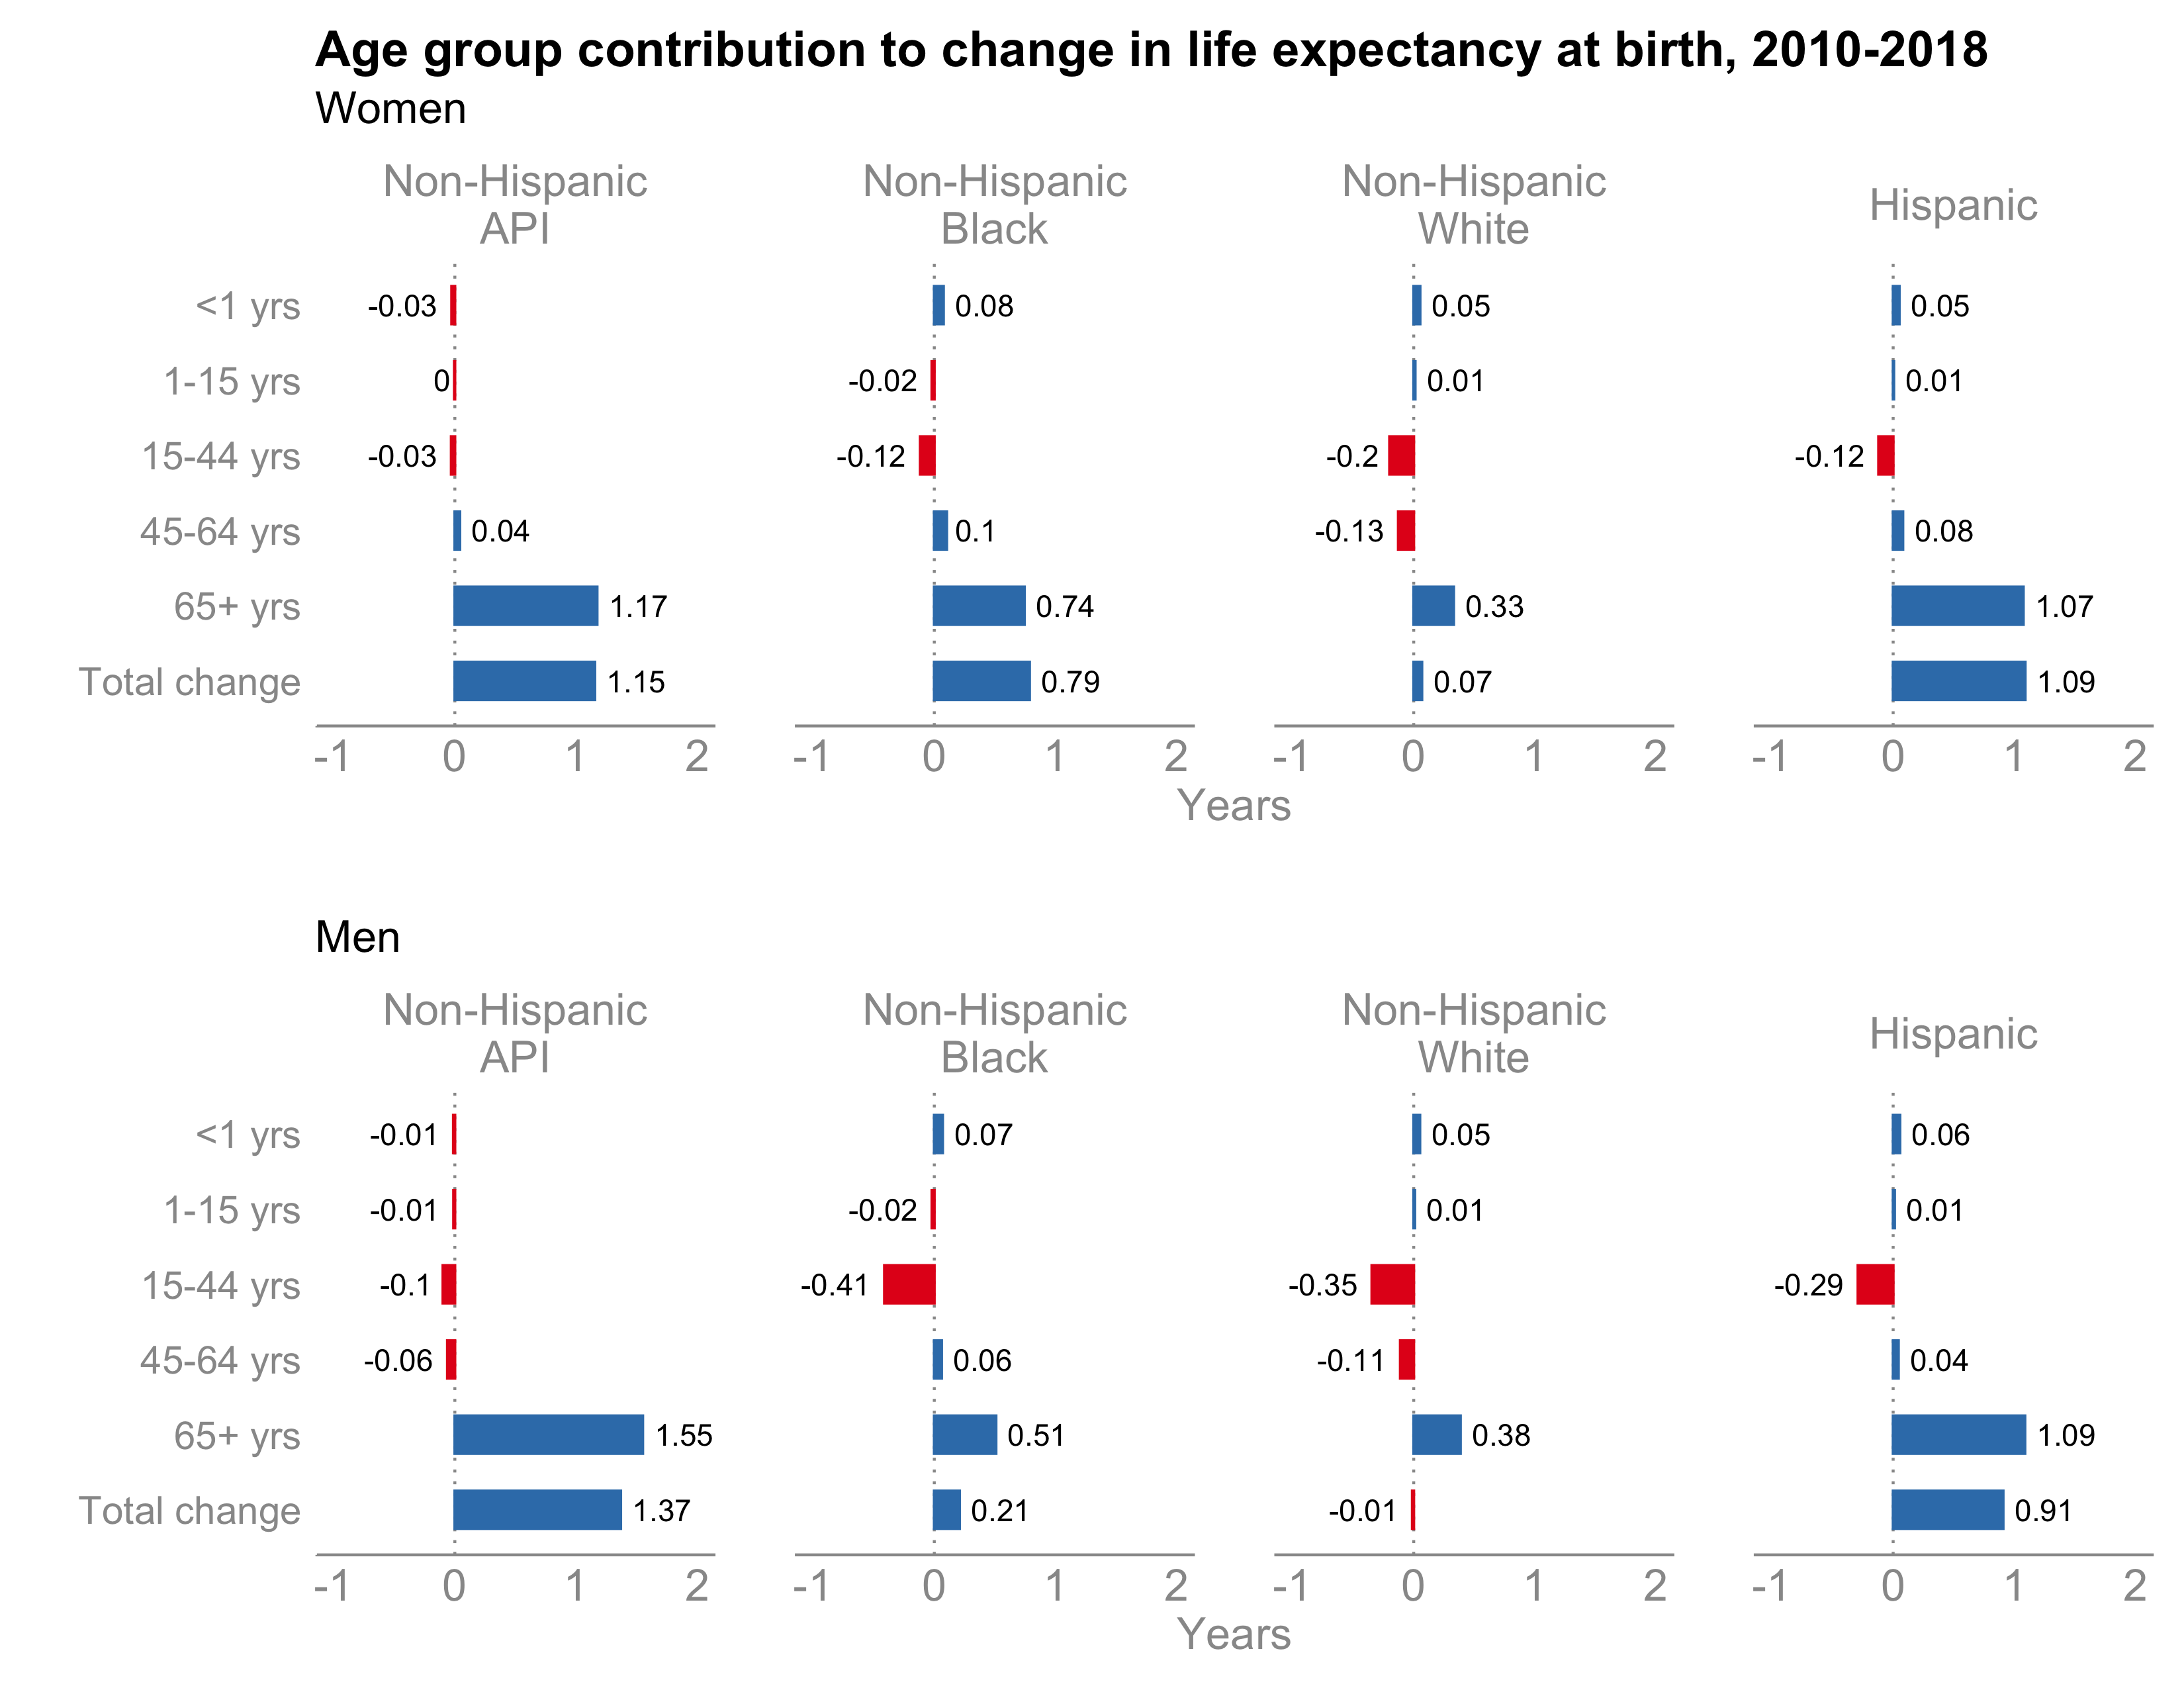
\includegraphics[width=1\linewidth]{../figures/le-age-decomp-2010-2018}

\newpage

\textbf{Supplemental Figure 8.} Age-adjusted death rates per 100,000 by
urban (purple) or rural (green) categorization, 1969-2016. Source:
Authors' calculations of data from SEER*Stat (National Cancer Institute
2019). Data: \url{https://osf.io/rj83e/} Code:
\url{https://osf.io/b856t/}

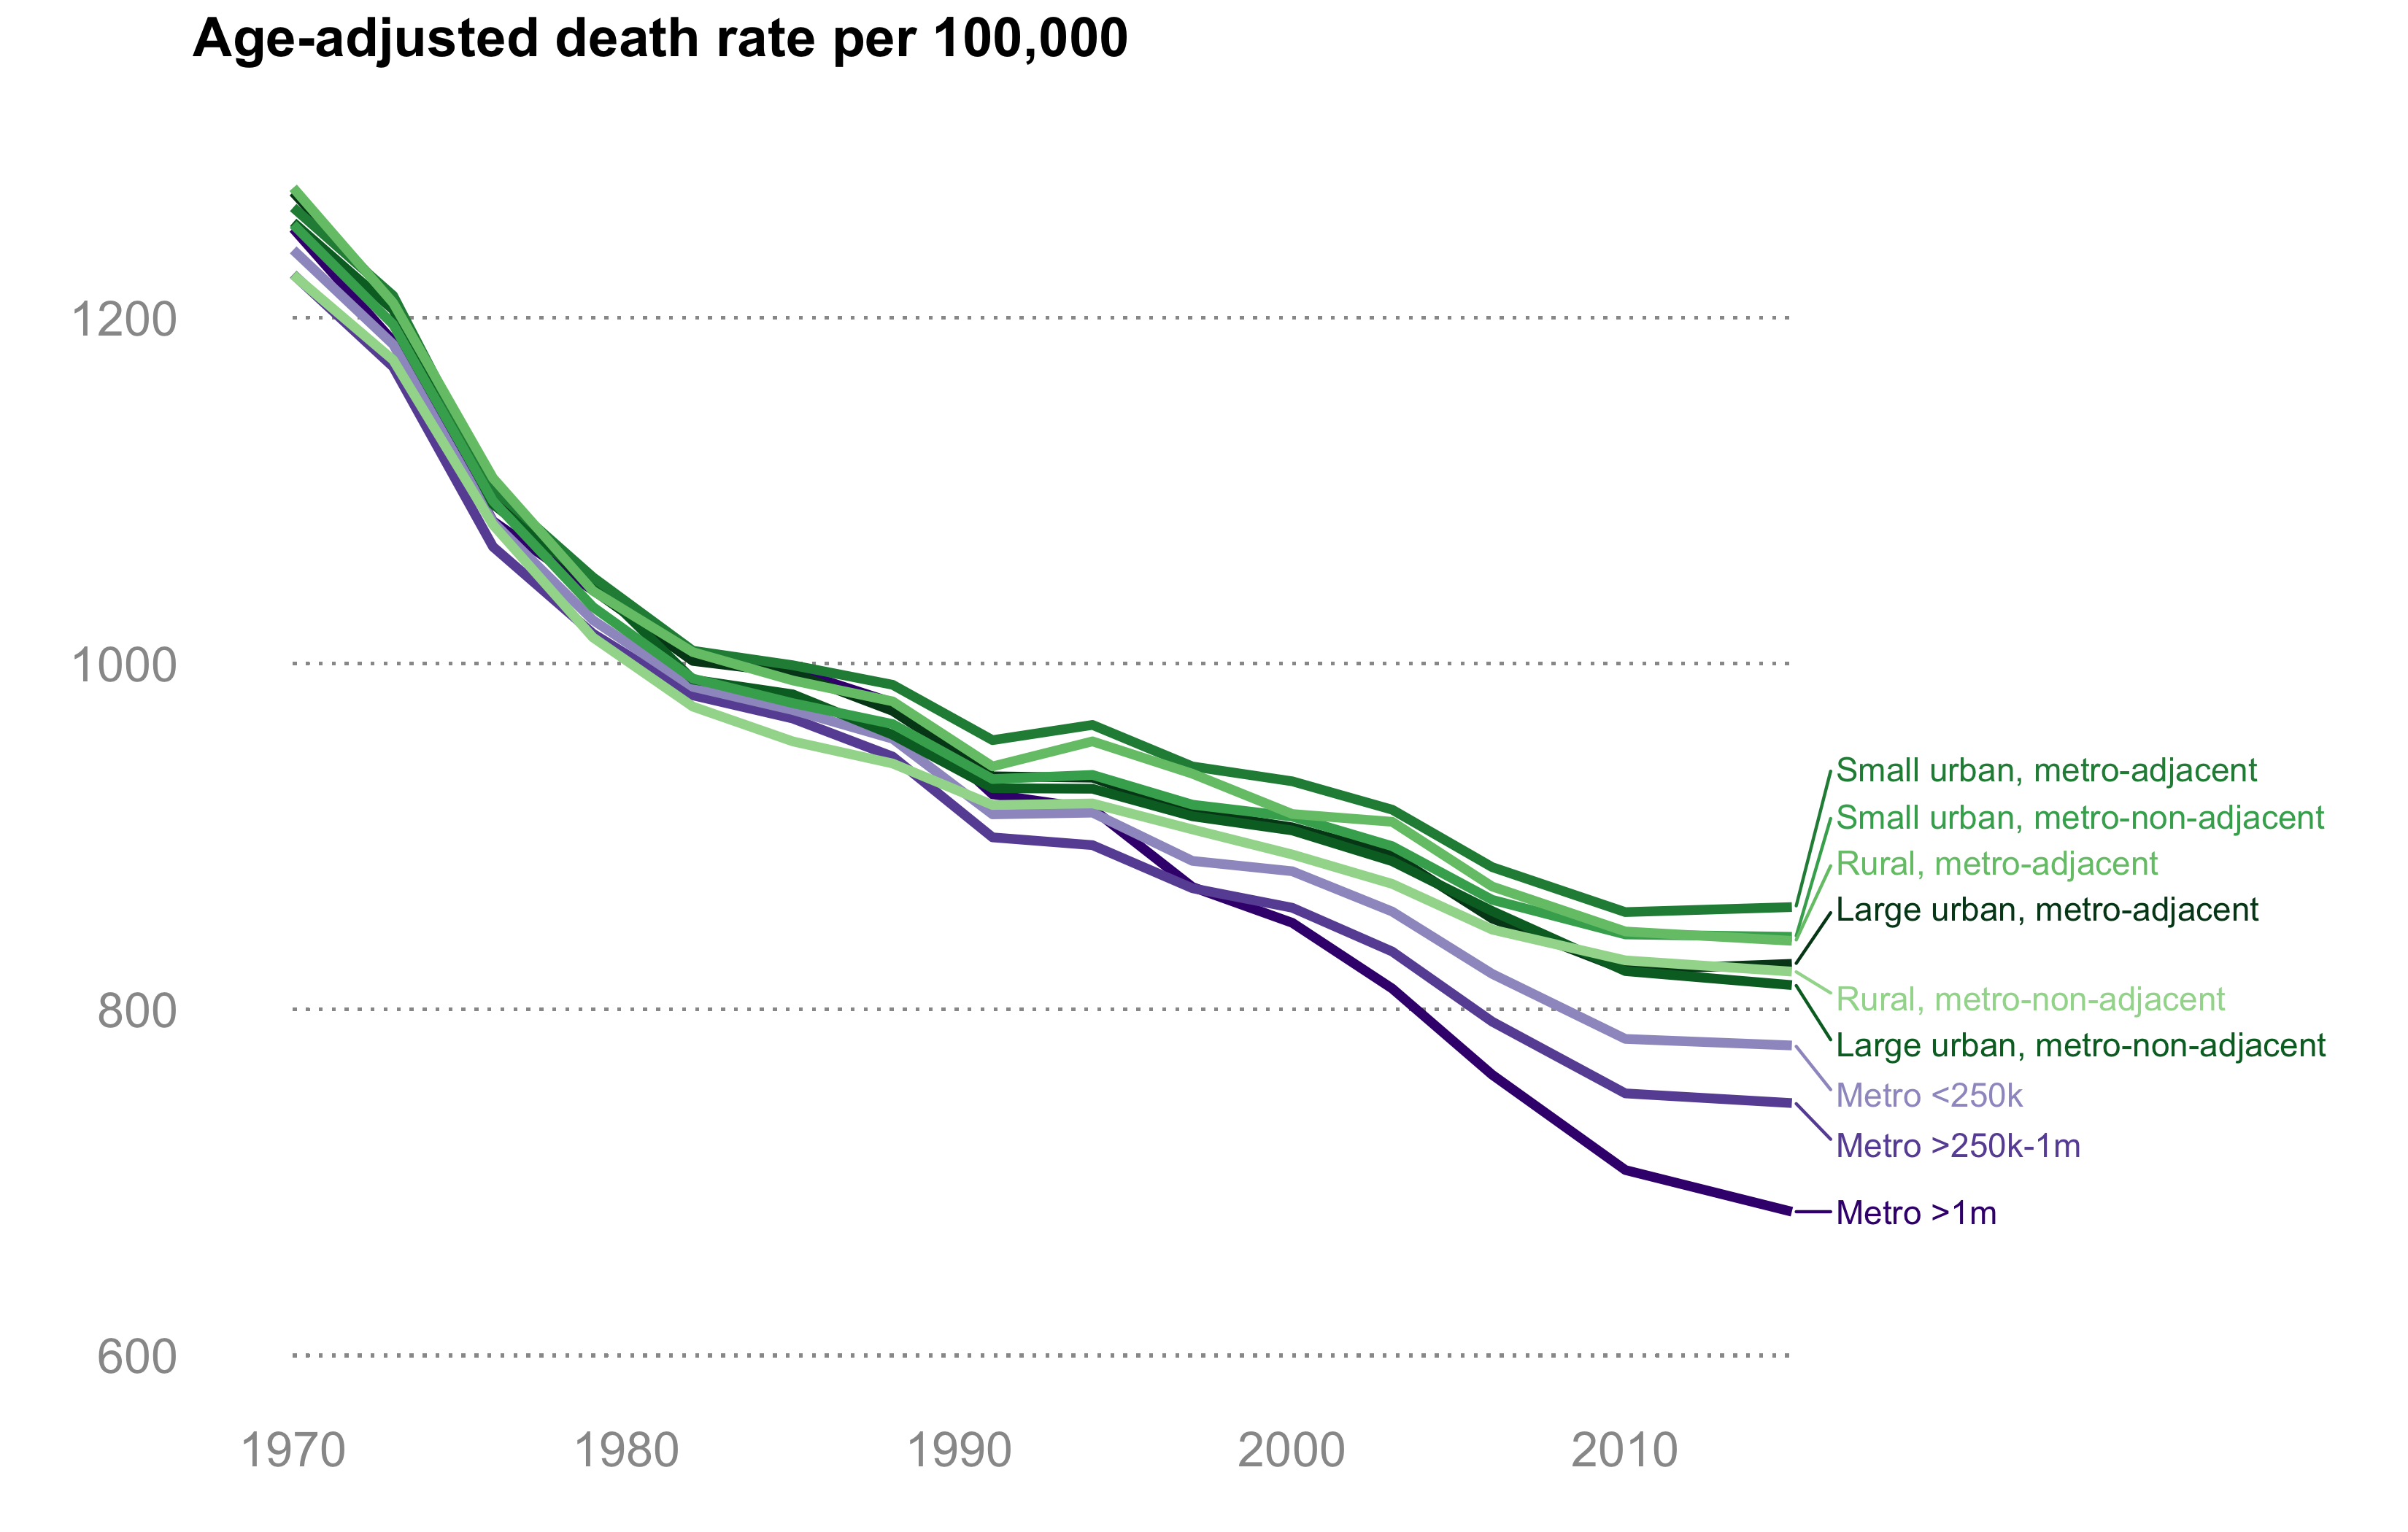
\includegraphics[width=1\linewidth]{../figures/rural-aadr-trends}

\newpage

\textbf{Supplemental Figure 9.} Decomposition of the urban-rural life
expectancy gap by cause-of-death, 1969-71 and 2012-16. Source: Authors'
calculations of data from SEER*Stat (National Cancer Institute 2019).
Data: \url{https://osf.io/rj83e/}, \url{https://osf.io/rwc68/}, Code:
\url{https://osf.io/4nezp/}, \url{https://osf.io/d23fz/}

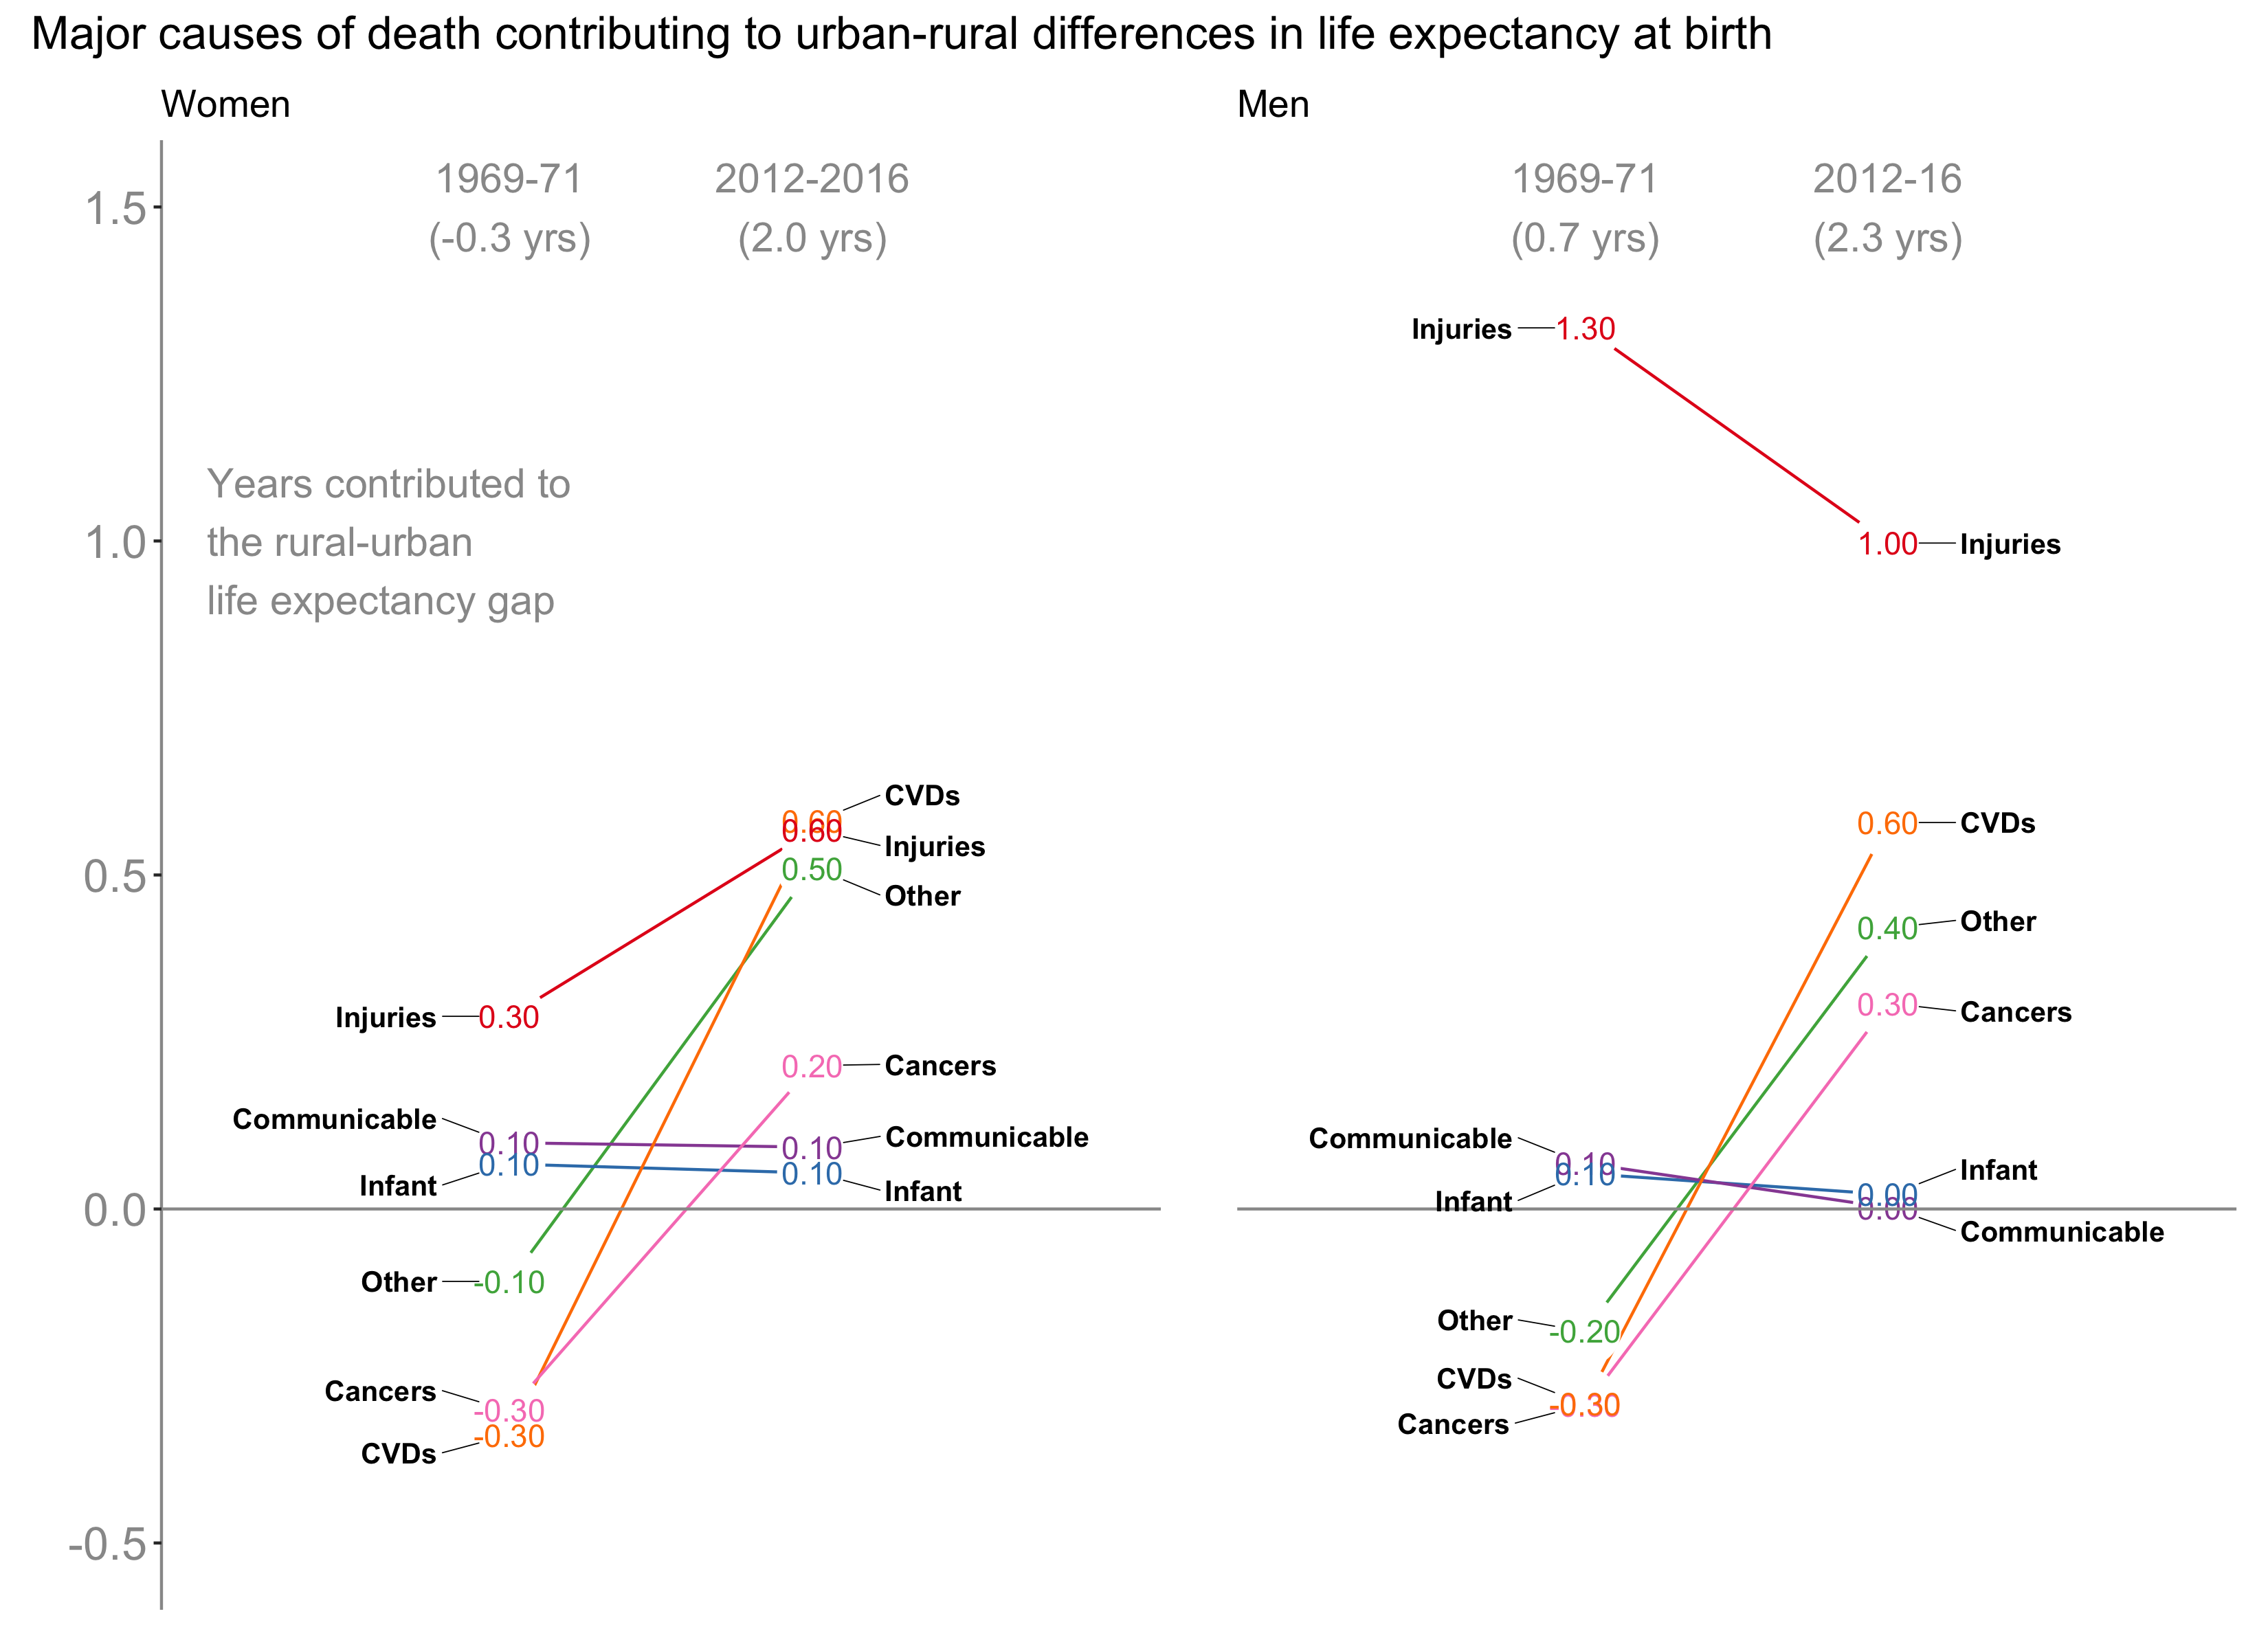
\includegraphics[width=1\linewidth]{../figures/ur-decomp-plot}

\newpage

\textbf{Supplemental Figure 10.} Trends in age-adjusted unintentional
poisoning death rates by urban-rural classification scheme, 1999-2018.
Source: Authors' calculations of data from SEER*Stat (National Cancer
Institute 2019). Data: \url{https://osf.io/zsbfw/} Code:
\url{https://osf.io/m7k2u/}

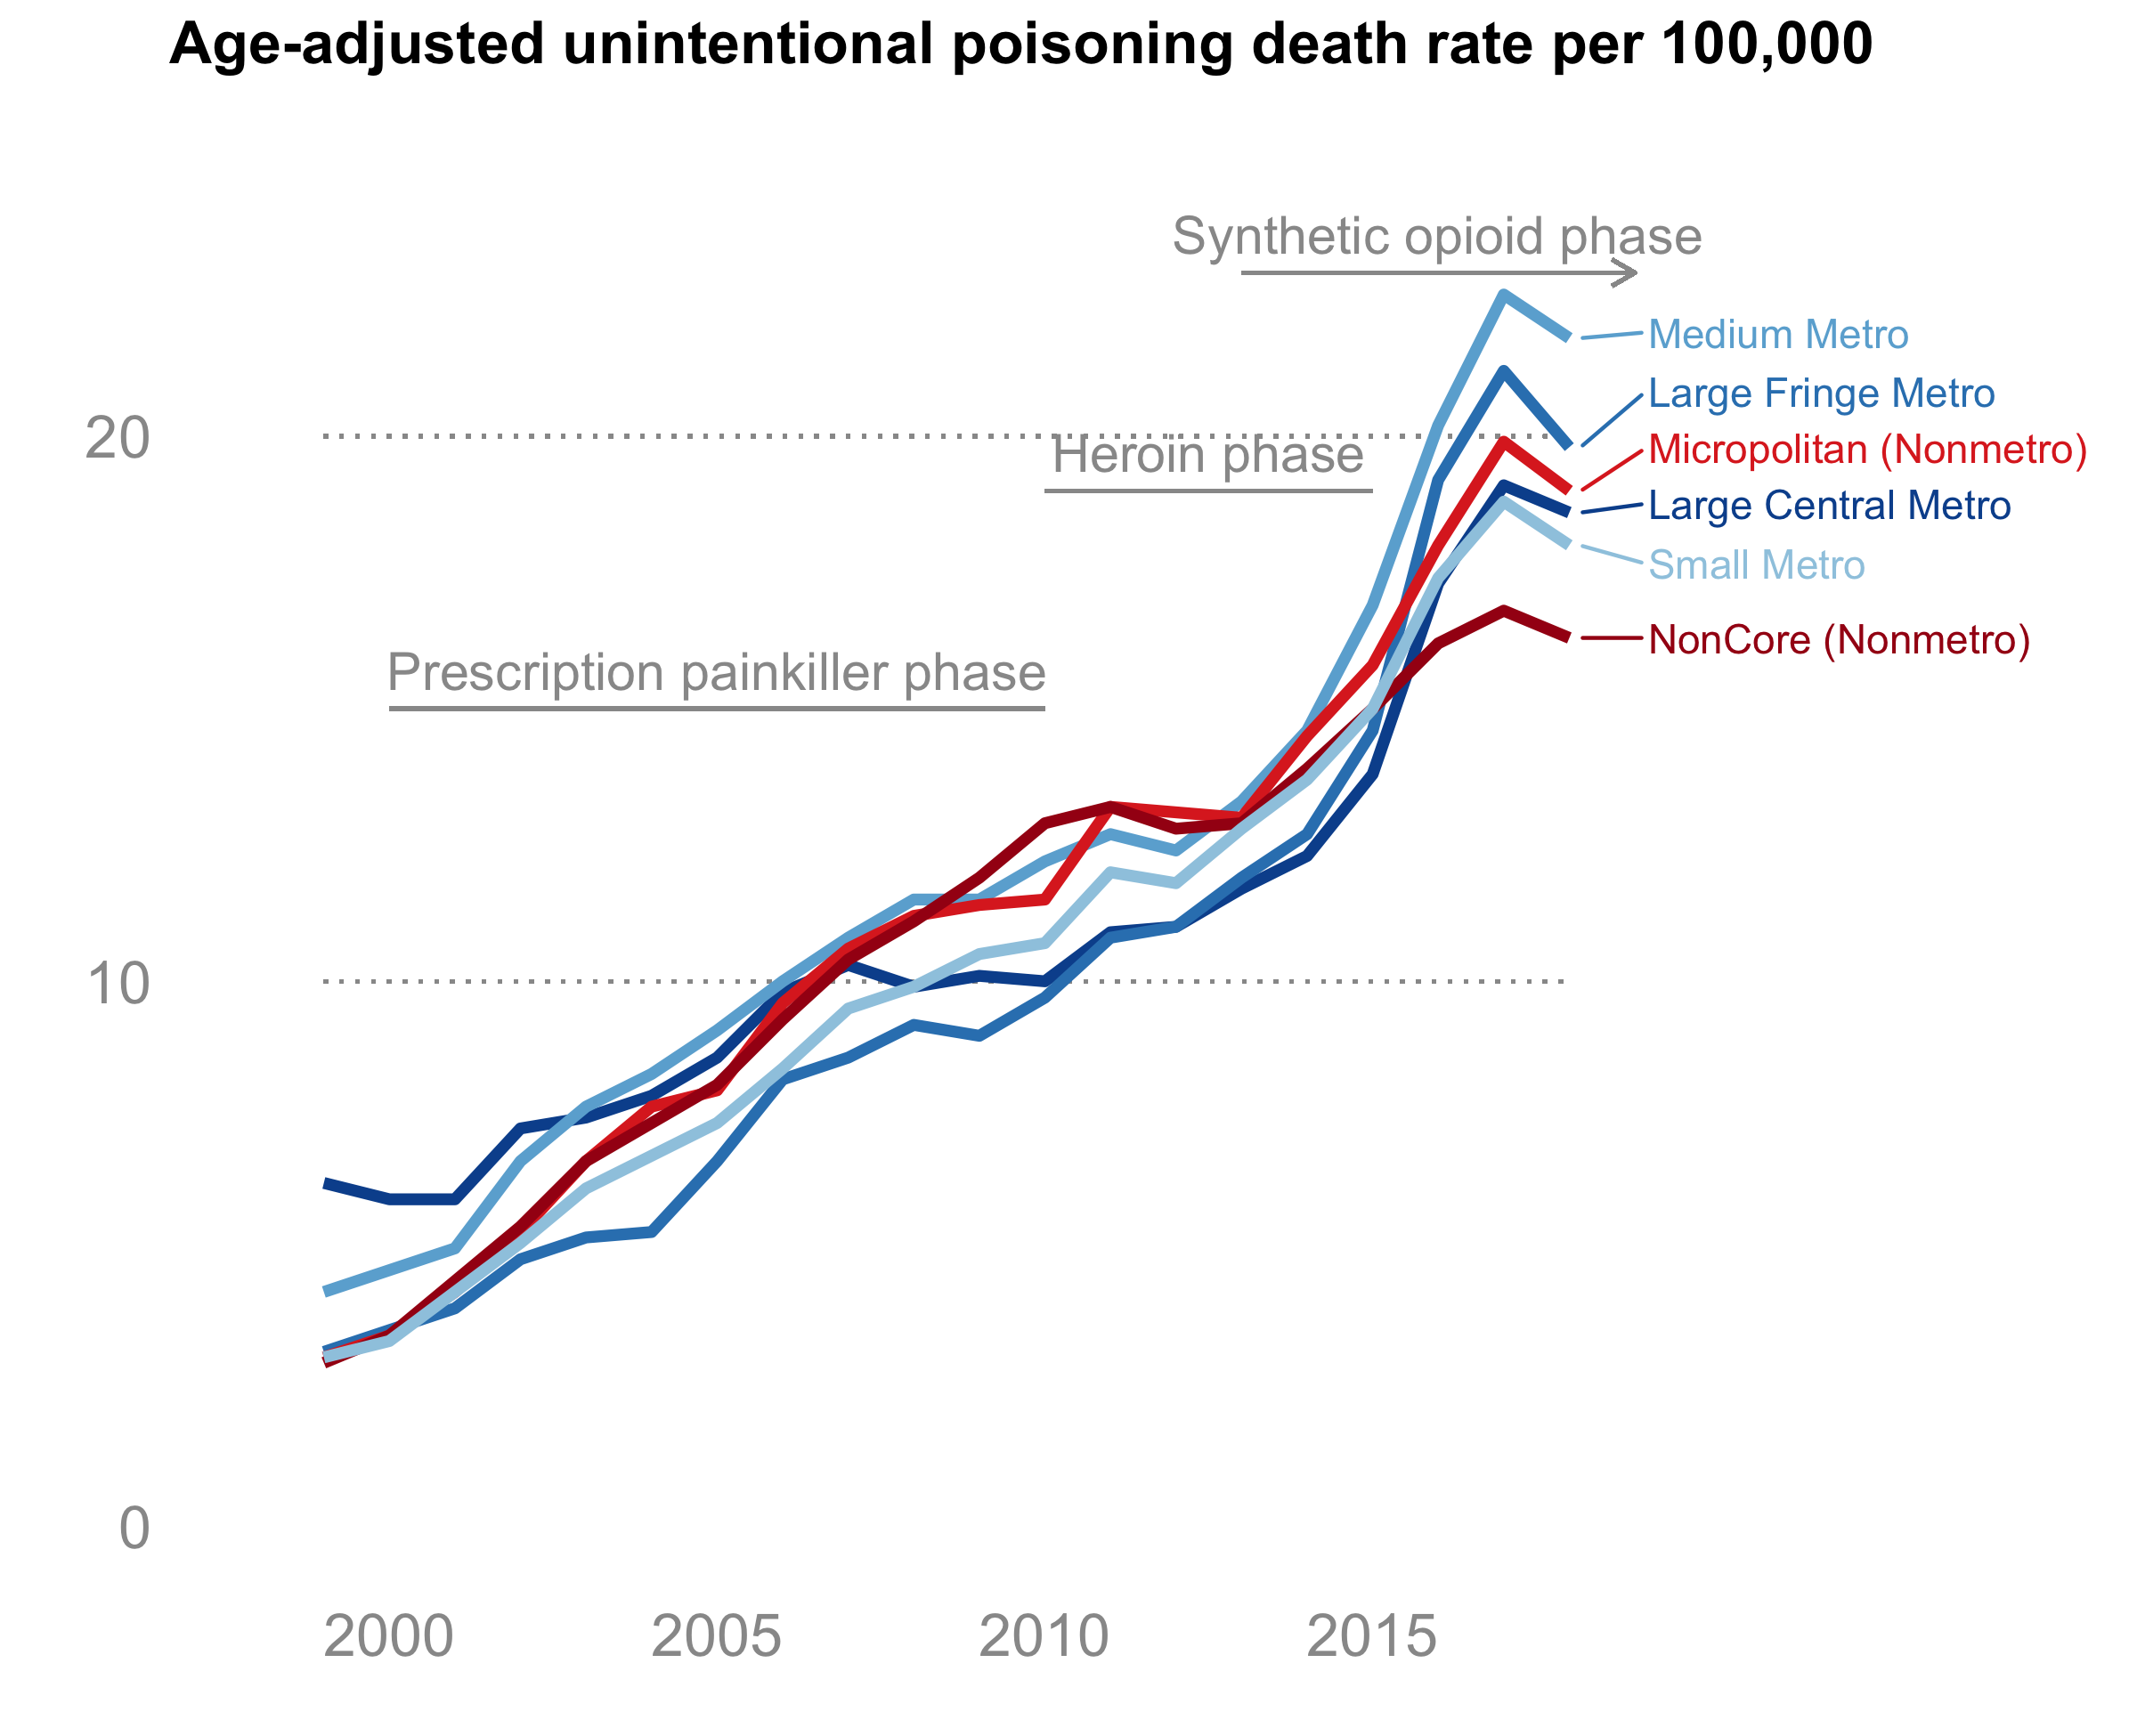
\includegraphics[width=1\linewidth]{../figures/rural-upoison-trends}

\newpage

\textbf{Supplemental Figure 11.} Trends in age-adjusted liver cancer
death rates by race-ethnicity and gender, 1999-2018. Source: Authors'
calculations of data from CDC WONDER (Centers for Disease Control and
Prevention and National Center for Health Statistics 2020). Data:
\url{https://osf.io/stj6a/}, \url{https://osf.io/d5jkh/} Code:
\url{https://osf.io/ybdmx/}

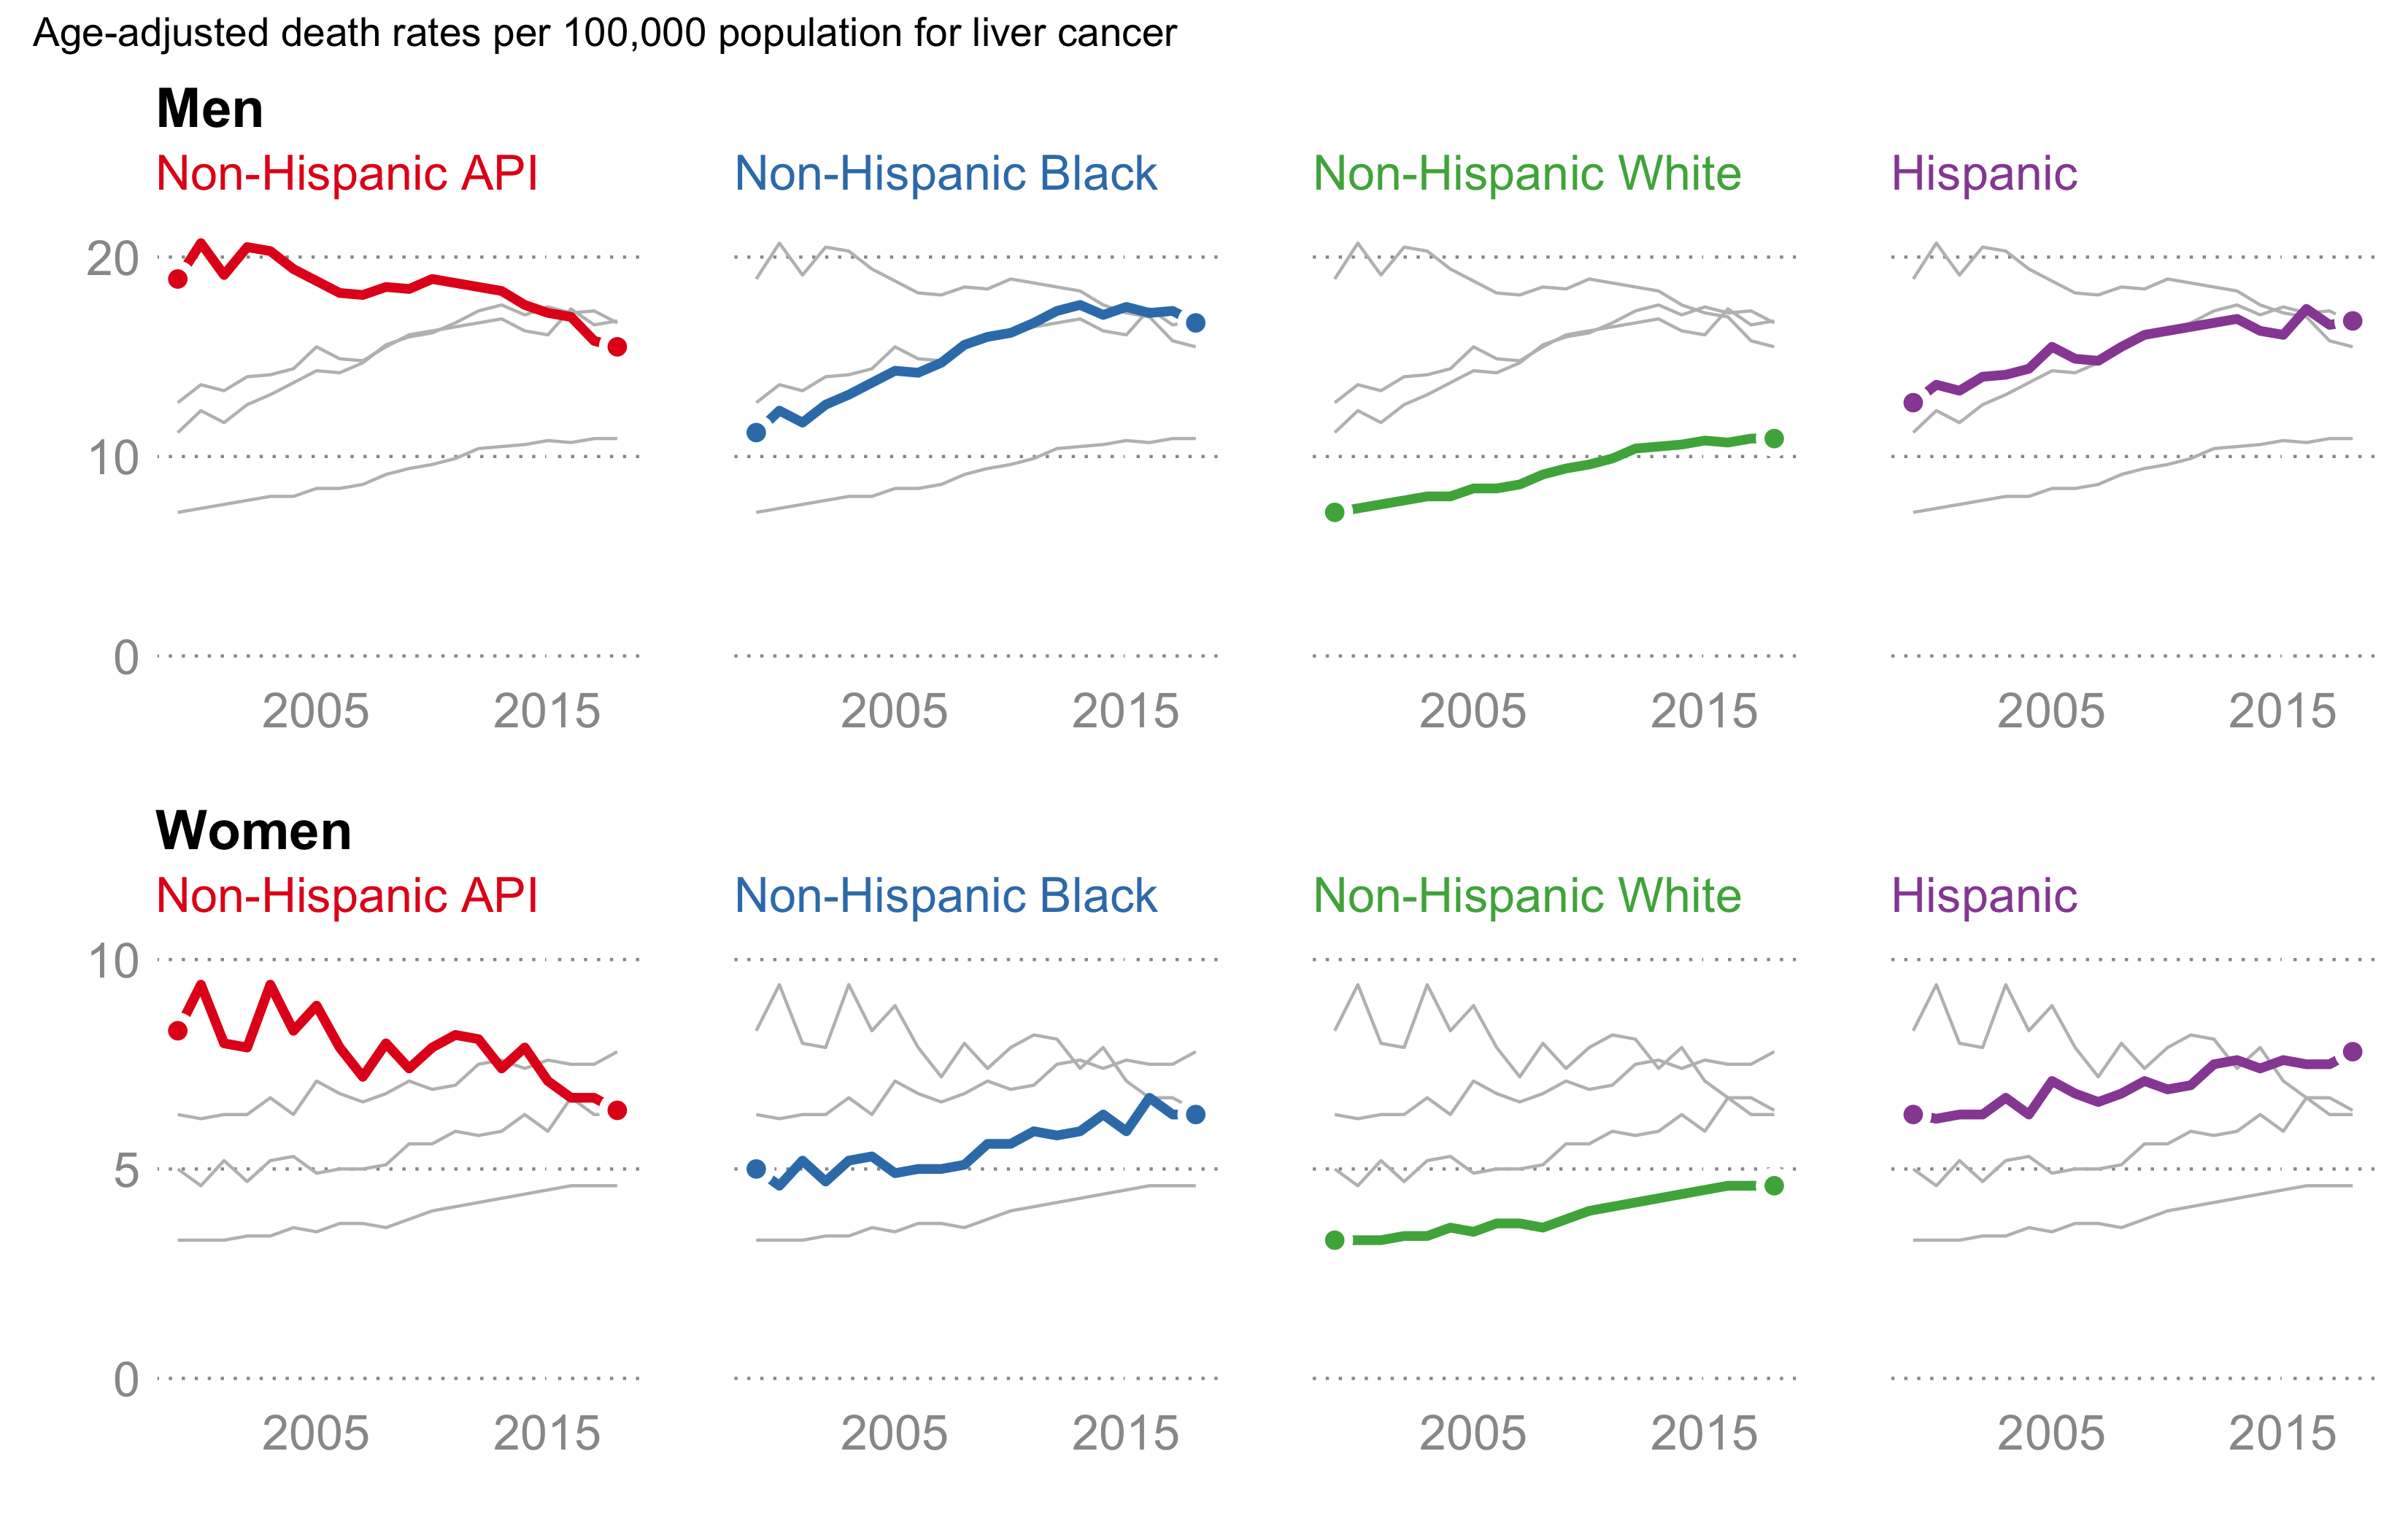
\includegraphics[width=1\linewidth]{../figures/liverca-race-trends}

\newpage

\textbf{Supplemental Figure 12.} Causes of death contributing to the
change in life expectancy at birth in the United States between 2010 and
2018, by gender and race-ethnicity. Red color indicates causes
contributing a decline, blue color indicates causes contributing an
increase. Source: Authors' calculations of data from CDC WONDER (Centers
for Disease Control and Prevention and National Center for Health
Statistics 2020). Data: \url{https://osf.io/tk8q3/},
\url{https://osf.io/mctx3/}, \url{https://osf.io/utdnv/} Code:
\url{https://osf.io/g9mp2/}, \url{https://osf.io/qd5w4/}

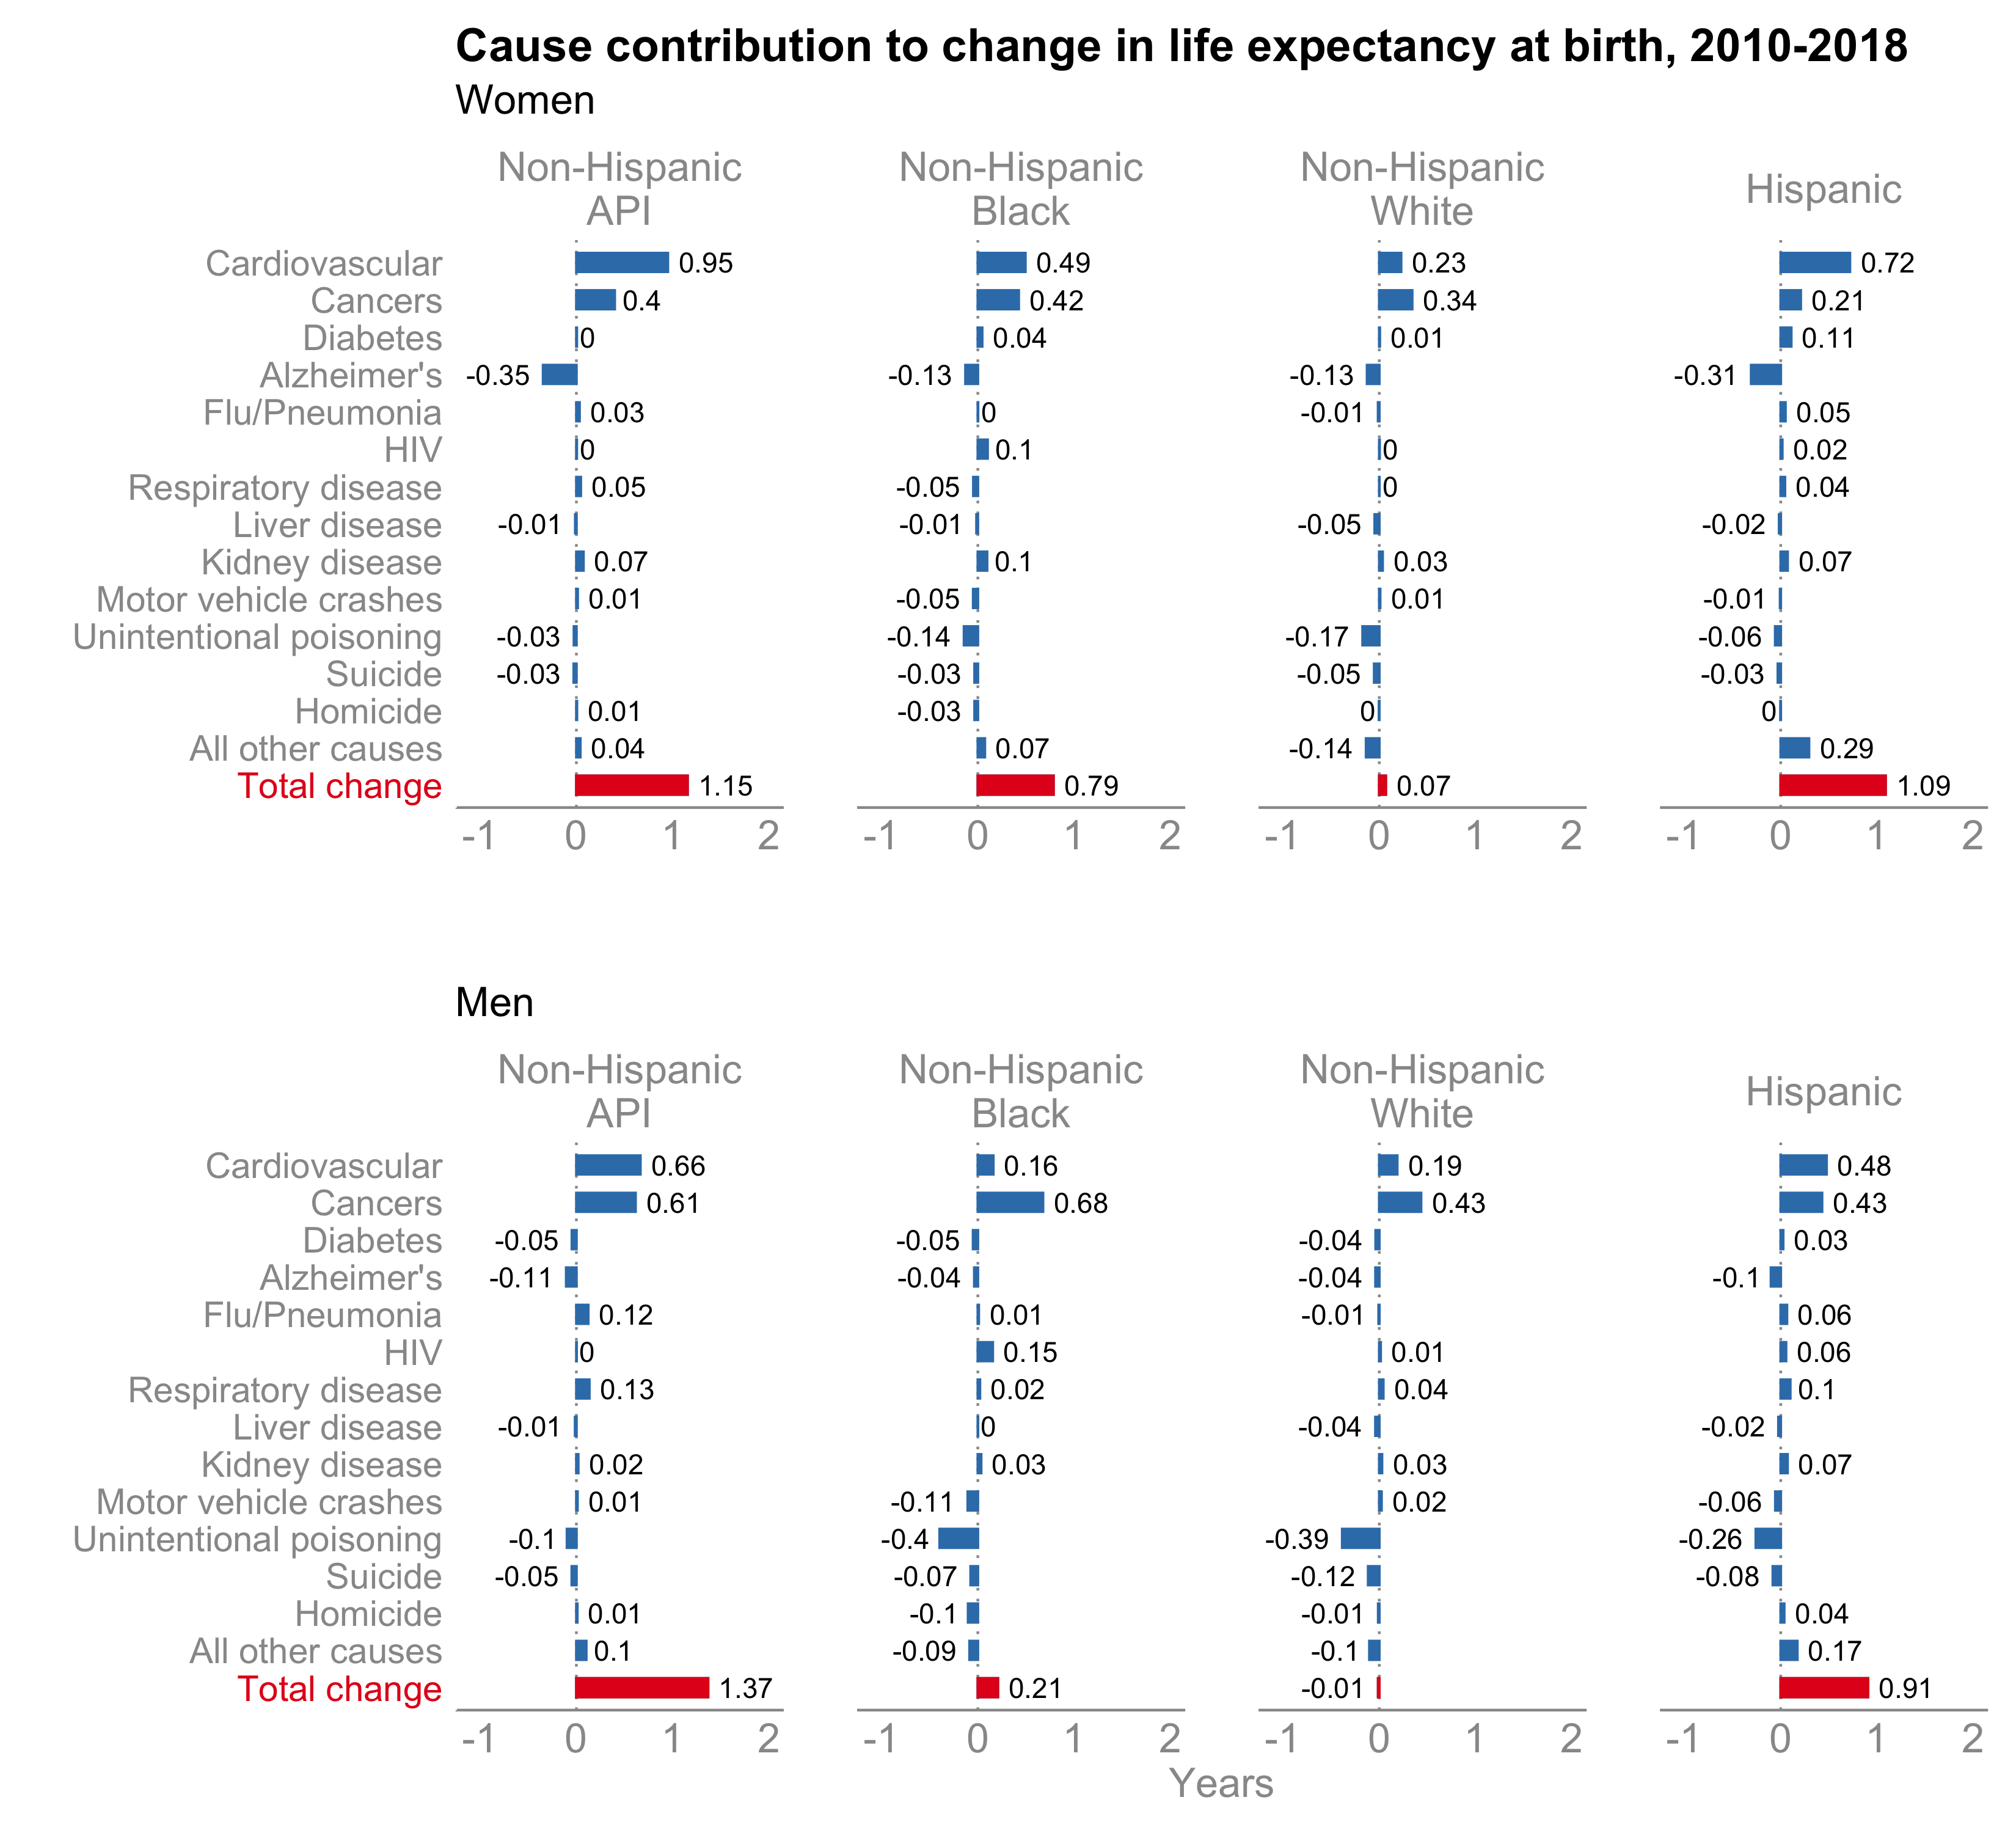
\includegraphics[width=1\linewidth]{../figures/le-cause-decomp-2010-2018}

\newpage

\textbf{Supplemental Figure 13.} Age-adjusted death rates per 100,000
for non-Hispanic white men aged 45-54, by state, 2010-2018. Source:
Authors' calculations of data from CDC WONDER (Centers for Disease
Control and Prevention and National Center for Health Statistics 2020).
Data: \url{https://osf.io/jn5ts/}, \url{https://osf.io/vdjbp/},
\url{https://osf.io/xpz6g/}, \url{https://osf.io/w9ady/} Code:
\url{https://osf.io/va4u7/}

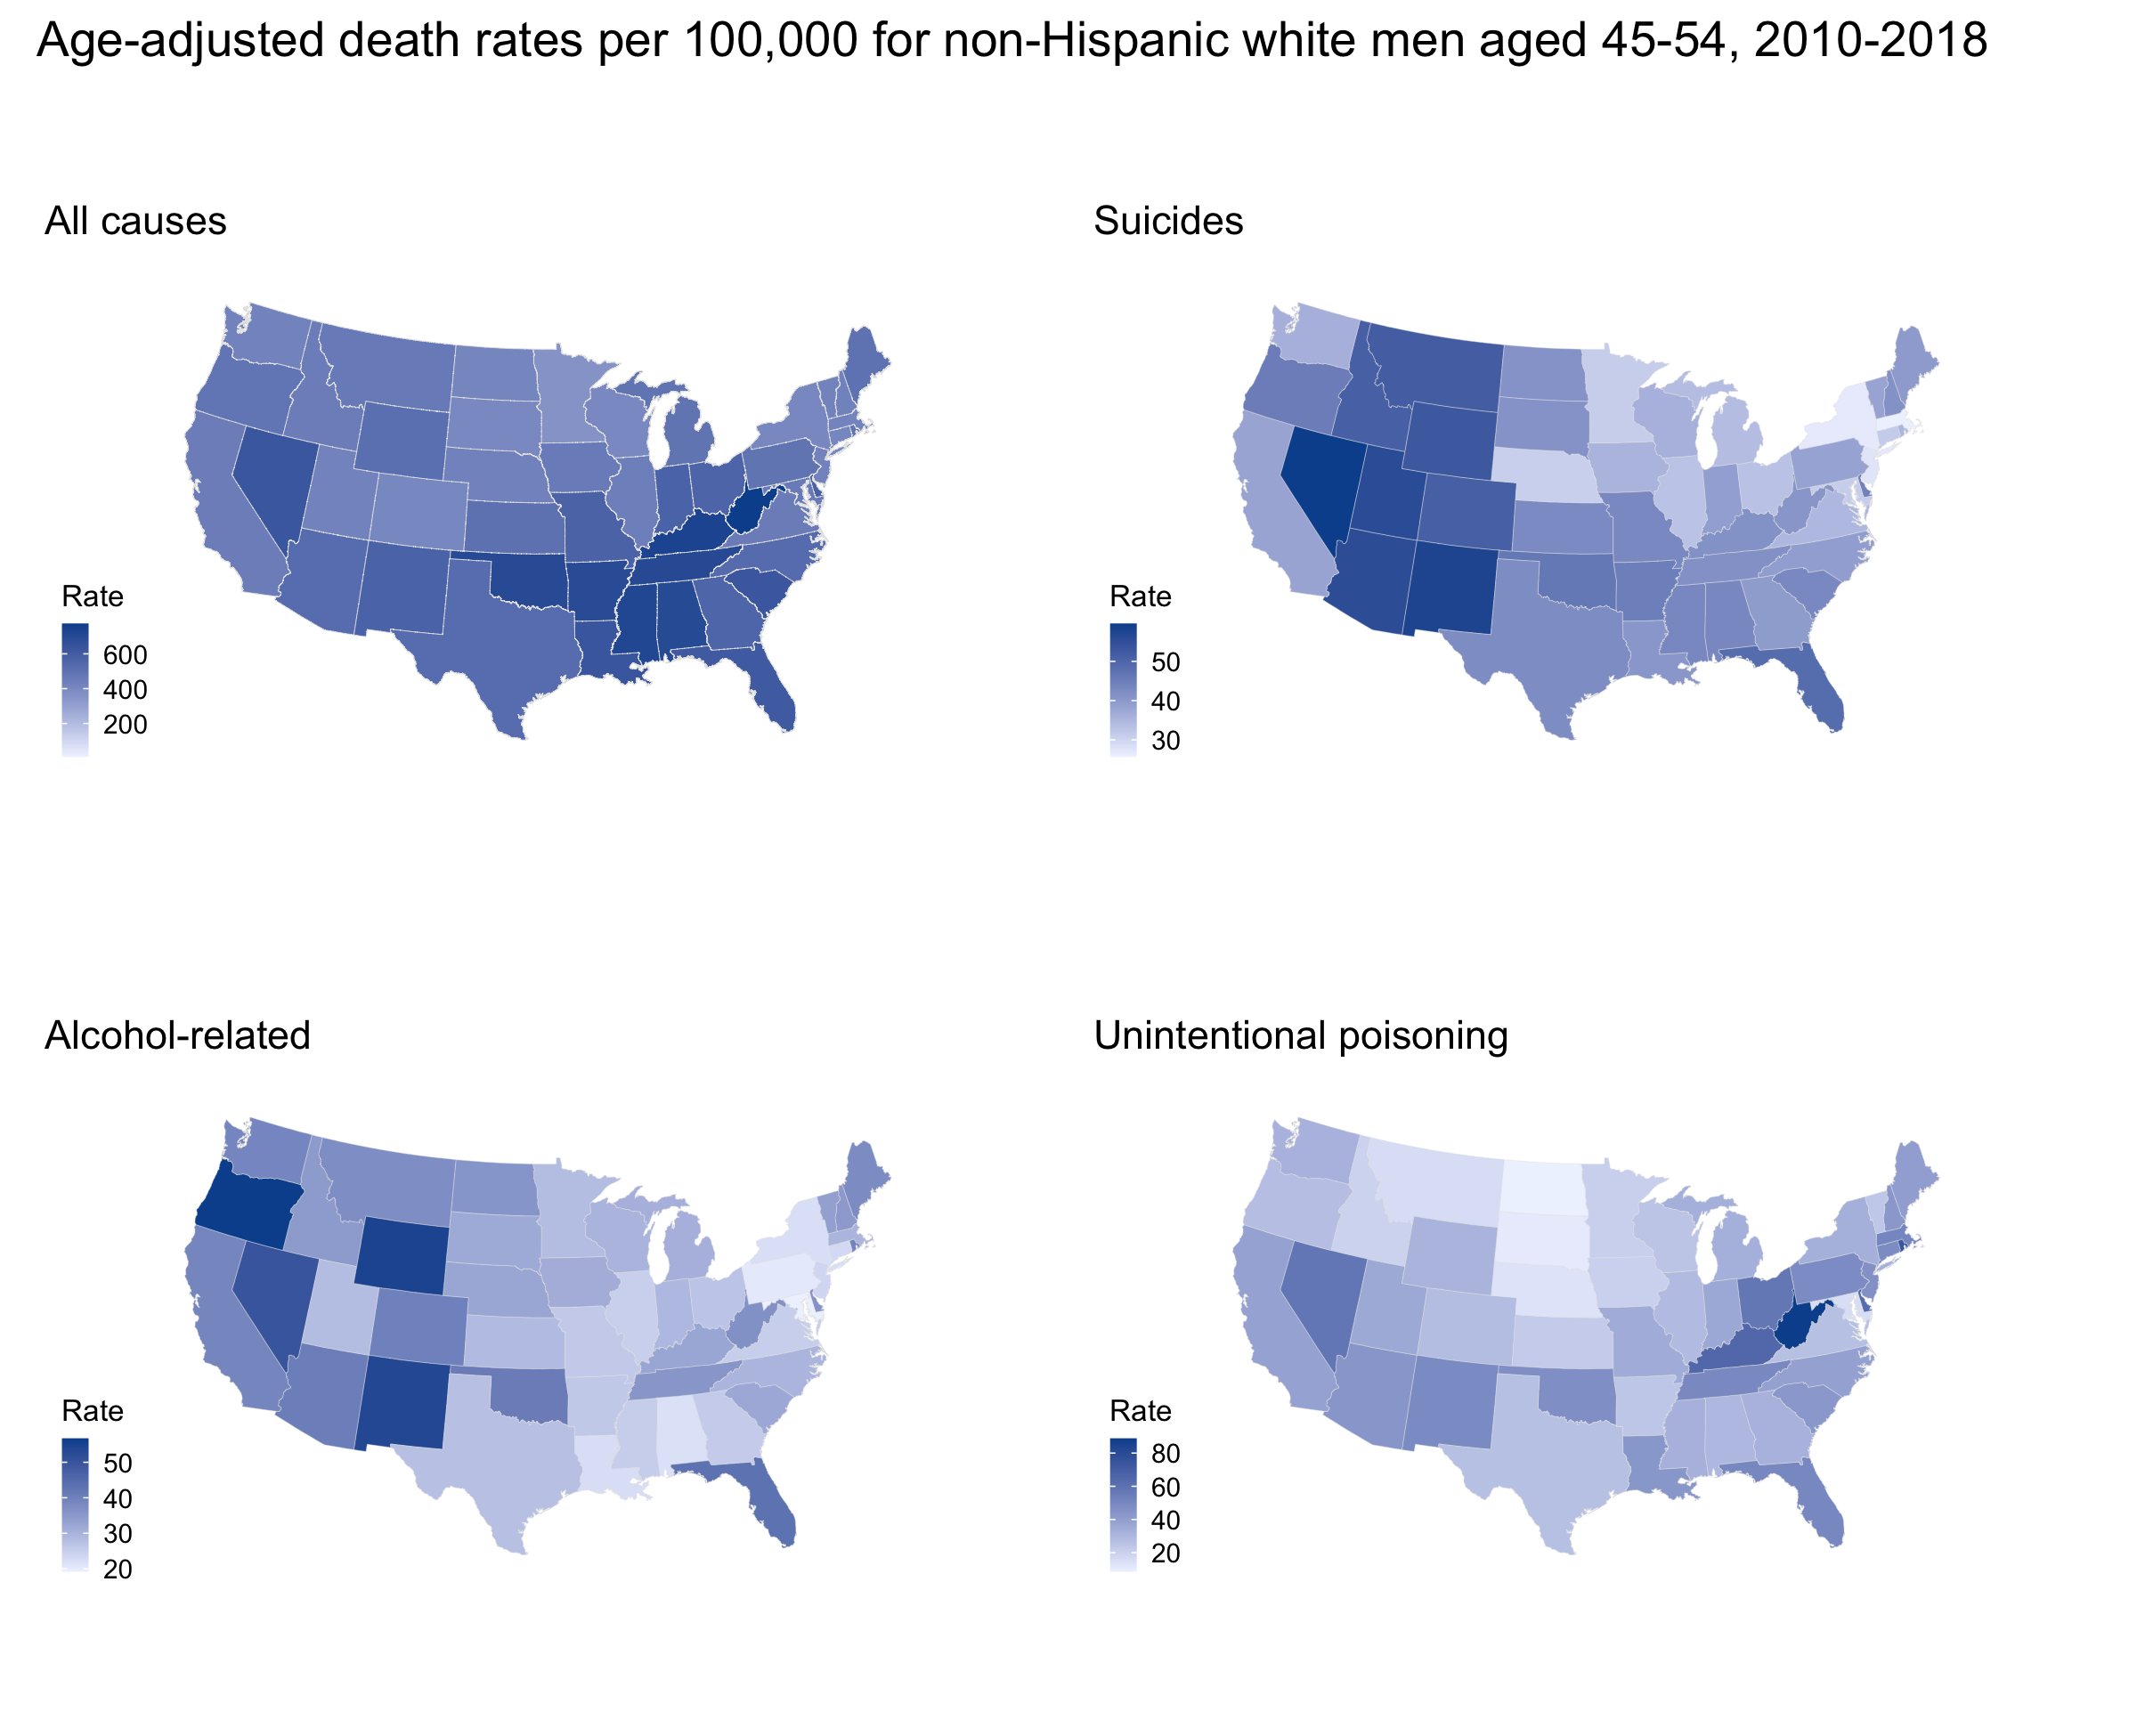
\includegraphics[width=1\linewidth]{../figures/nhwm-45-54-maps}

\newpage

\hypertarget{literature-cited}{%
\section*{\textbar{} LITERATURE CITED}\label{literature-cited}}
\addcontentsline{toc}{section}{\textbar{} LITERATURE CITED}

\hypertarget{refs}{}
\leavevmode\hypertarget{ref-arias2016}{}%
Arias, Elizabeth, Melonie Heron, National Center for Health Statistics,
Jahn Hakes, and US Census Bureau. 2016. ``The Validity of Race and
Hispanic-Origin Reporting on Death Certificates in the United States: An
Update.'' \emph{Vital and Health Statistics. Series 2, Data Evaluation
and Methods Research}, no. 172 (January): 1--21.

\leavevmode\hypertarget{ref-arias2008}{}%
Arias, Elizabeth, William S. Schauman, Karl Eschbach, Paul D. Sorlie,
and Eric Backlund. 2008. ``The Validity of Race and Hispanic Origin
Reporting on Death Certificates in the United States.'' \emph{Vital and
Health Statistics. Series 2, Data Evaluation and Methods Research}, no.
148 (October): 1--23.

\leavevmode\hypertarget{ref-arriaga1989}{}%
Arriaga, Eduardo E. 1989. ``Changing Trends in Mortality Decline During
the Last Decades.'' In \emph{Differential Mortality: Methodological
Issues and Biosocial Factors}, edited by LT Ruzicka, GJ Wunsch, and P
Kane, 105--29. Oxford, England: Clarendon Press.

\leavevmode\hypertarget{ref-arriaga1984}{}%
---------. 1984. ``Measuring and Explaining the Change in Life
Expectancies.'' \emph{Demography} 21 (1): 83--96.
\url{https://doi.org/10.2307/2061029}.

\leavevmode\hypertarget{ref-wonder2020}{}%
Centers for Disease Control and Prevention, and National Center for
Health Statistics. 2020. ``Underlying Cause of Death, 1999-2018 on CDC
WONDER Online Database, Released in 2020. Data Are from the Multiple
Cause of Death Files, 1999-2018.''
https://wonder.cdc.gov/ucd-icd10.html.

\leavevmode\hypertarget{ref-kim2000}{}%
Kim, H. J., M. P. Fay, E. J. Feuer, and D. N. Midthune. 2000.
``Permutation Tests for Joinpoint Regression with Applications to Cancer
Rates.'' \emph{Statistics in Medicine} 19 (3): 335--51.
\url{https://doi.org/10.1002/(sici)1097-0258(20000215)19:3\%3C335::aid-sim336\%3E3.0.co;2-z}.

\leavevmode\hypertarget{ref-kochanek2019}{}%
Kochanek, Kenneth D., Sherry L. Murphy, Jiaquan Xu, and Elizabeth Arias.
2019. ``Deaths: Final Data for 2017.'' \emph{National Vital Statistics
Reports: From the Centers for Disease Control and Prevention, National
Center for Health Statistics, National Vital Statistics System} 68 (9):
1--77.

\leavevmode\hypertarget{ref-nci2019}{}%
National Cancer Institute. 2019. ``SEER*Stat Version 8.3.6. SEER*Stat
Database: Mortality - All COD, Aggregated with County, Total U.S.
(1969-2017) - Linked to County Attributes - Total U.S., 1969-2018
Counties.'' Hyattsville, Maryalnd: National Cancer Institute,
Surveillance Research Program.

\leavevmode\hypertarget{ref-nci2020}{}%
---------. 2020. ``Joinpoint Regression Program, Version 4.8.0.1.''
Hyattsville, Maryalnd: National Cancer Institute, Surveillance Research
Program.

\leavevmode\hypertarget{ref-preston2001}{}%
Preston, Samuel H., Patrick Heuveline, and Michel Guillot. 2001.
\emph{Demography: Measuring and Modeling Population Processes}. Malden,
Mass.: Blackwell.

\leavevmode\hypertarget{ref-theworldbankgroup2020}{}%
The World Bank Group. 2020. ``World Development Indicators \textbar{}
DataBank.''
https://databank.worldbank.org/source/world-development-indicators.

\leavevmode\hypertarget{ref-woolf2019}{}%
Woolf, Steven H., and Heidi Schoomaker. 2019. ``Life Expectancy and
Mortality Rates in the United States, 1959-2017.'' \emph{JAMA} 322 (20):
1996--2016. \url{https://doi.org/10.1001/jama.2019.16932}.

\end{document}
